\documentclass[12pt,spanish,fleqn,openany,letterpaper,pagesize]{scrbook}

\usepackage[ansinew]{inputenc}
\usepackage[spanish]{babel}
\usepackage{fancyhdr}
\usepackage{epsfig}
\usepackage{epic}
\usepackage{eepic}
\usepackage{amsmath}
\usepackage{threeparttable}
\usepackage{amscd}
\usepackage{here}
\usepackage{graphicx}
\usepackage{lscape}
\usepackage{tabularx}
\usepackage{subfigure}
\usepackage{longtable}
\usepackage{enumitem}
\usepackage{amsfonts}

\usepackage{rotating} %Para rotar texto, objetos y tablas seite. No se ve en DVI solo en PS. Seite 328 Hundebuch
                        %se usa junto con \rotate, \sidewidestable ....




\pagestyle{fancyplain}%\addtolength{\headwidth}{\marginparwidth}

\textheight23cm \topmargin0cm \textwidth16.5cm%altura del texto  margen superior y ancho

\oddsidemargin0.5cm \evensidemargin-0.5cm% Margenes en pagina par e impar

\renewcommand{\chaptermark}[1]{\markboth{\thechapter\; #1}{}}
\renewcommand{\sectionmark}[1]{\markright{\thesection\; #1}}

\lhead[\fancyplain{}{\thepage}]{\fancyplain{}{\rightmark}}
\rhead[\fancyplain{}{\leftmark}]{\fancyplain{}{\thepage}}

\fancyfoot{}
\thispagestyle{fancy}%

%
\setlength{\parindent}{1cm}


%Para tablas,  redefine el backschlash en tablas donde se define la posici\'{o}n del texto en las
%casillas (con \centering \raggedright o \raggedleft)
%\newcommand{\PreserveBackslash}[1]{\let\temp=\\#1\let\\=\temp}
%\let\PBS=\PreserveBackslash

%Espacio entre lineas
\renewcommand{\baselinestretch}{1.5}


%espacio entre parrafos
\setlength{\parskip}{0.5cm}

%New command for the table properties of the activated carbon
\newcommand{\arr}[1]{\raisebox{1.5ex}[0cm][0cm]{#1}}






%\usepackage[utf8x]{inputenx}
\usepackage{amssymb}
\usepackage{listings}
\usepackage{xcolor}
\usepackage{array}
\usepackage{graphicx}
\graphicspath{ {img/} }
\usepackage{wrapfig}
\usepackage[rightcaption]{sidecap}
\usepackage{booktabs}
\usepackage{verbatim}
\usepackage{multirow}
\usepackage{pdfpages}
\usepackage{float}
\usepackage{lmodern}
\usepackage{caption}
\usepackage{sansmath}

\captionsetup[figure]{font=small,labelfont=small}

        
%paquetes para poner 2 imagenes lado a lado




\begin{document}
\pagenumbering{roman}
%\newpage
%\setcounter{page}{1}
\begin{center}
\begin{figure}
\centering%

\epsfig{file=HojaTitulo/EscudoUN.eps,scale=1}%
\end{figure}
\thispagestyle{empty} \vspace*{2.0cm} \textbf{\huge
An\'{a}lisis tridimensional de equilibrio l\'{i}mite por movimientos en masa para la cuenca hidrogr\'{a}fica de la quebrada La Linda en la vereda Monte Loro en Ciudad Bolivar (Antioquia) mediante el programa Scoops 3D}\\[6.0cm]
\Large\textbf{Juan Felipe Luj\'{a}n Rivas}\\[6.0cm]
\small Universidad Nacional de Colombia\\
Facultad de Minas, Departamento de ingenier\'{i}a Civil )\\
Medell\'{i}n, Colombia\\
2017\\
\end{center}

\newpage{\pagestyle{empty}\cleardoublepage}

\newpage
\begin{center}
\thispagestyle{empty} \vspace*{0cm} \textbf{\huge
An\'{a}lisis tridimensional de equilibrio l\'{i}mite por movimientos en masa para la cuenca hidrogr\'{a}fica de la quebrada La Linda en la vereda Monte Loro en Ciudad Bolivar (Antioquia) mediante el programa Scoops 3D}\\[3.0cm]
\Large\textbf{Juan Felipe Luj\'{a}n Rivas}\\[3.0cm]
\small Tesis o trabajo de grado presentada(o) como requisito parcial para optar al
t\'{\i}tulo de:\\
\textbf{ Magister en Ingenier\'{\i}a Geotecnia}\\[2.5cm]
Director(a):\\
Ph.D. Ludger O. Suarez. Burgoa\\[2.0cm]
L\'{\i}nea de Investigaci\'{o}n:\\
Estabilidad de Laderas\\
Grupo de Investigaci\'{o}n:\\
Grupo de Investigaci\'{o}n BIMs (Blocks in Matrix)\\[2.5cm]
Universidad Nacional de Colombia\\
Facultad de Minas, Departamento de Ingenier\'{i}a Civil\\
Medell\'in, Colombia\\
2017\\
\end{center}

\newpage{\pagestyle{empty}\cleardoublepage}

\newpage
\thispagestyle{empty} \textbf{}\normalsize
\\\\\\%
\textbf{(Dedicatoria o un lema)}\\[4.0cm]

\begin{flushright}
\begin{minipage}{8cm}
    \noindent
        \small
        Su uso es opcional y cada autor podr\'{a} determinar la distribuci\'{o}n del texto en la p\'{a}gina, se sugiere esta presentaci\'{o}n. En ella el autor dedica su trabajo en forma especial a personas y/o entidades.\\[1.0cm]\\
        Por ejemplo:\\[1.0cm]
        A mis padres\\[1.0cm]\\
        o\\[1.0cm]
        La preocupaci\'{o}n por el hombre y su destino siempre debe ser el
        inter\'{e}s primordial de todo esfuerzo t\'{e}cnico. Nunca olvides esto
        entre tus diagramas y ecuaciones.\\\\
        Albert Einstein\\
\end{minipage}
\end{flushright}

\newpage{\pagestyle{empty}\cleardoublepage}

\newpage
\thispagestyle{empty} \textbf{}\normalsize
\\\\\\%
\addcontentsline{toc}{chapter}{\numberline{}Agradecimientos}\\\\
\begin{figure}[H]
\centering
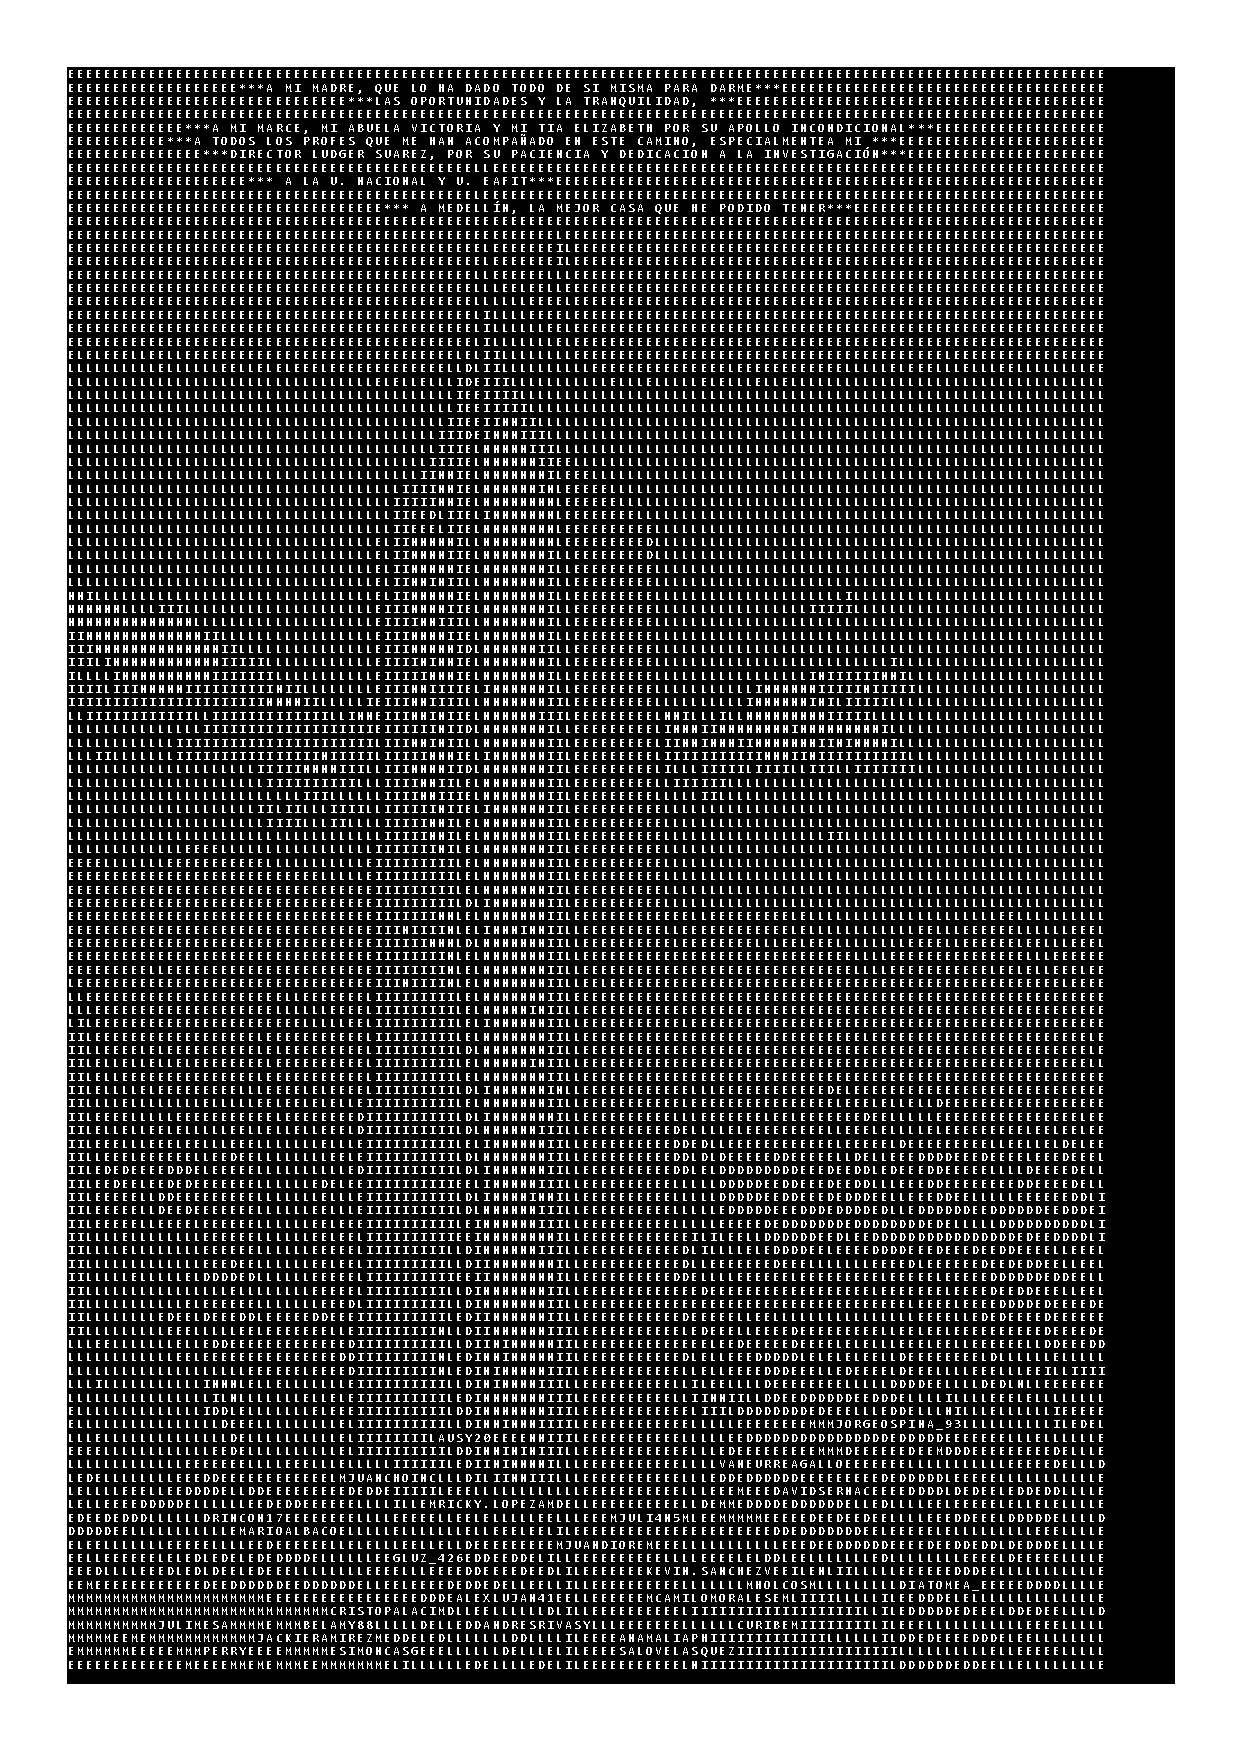
\includegraphics[trim={0 0.1cm 2.2cm 0},clip,scale=0.8]{img/dedicatoria/dedicatoria.pdf}
\end{figure}

\newpage{\pagestyle{empty}\cleardoublepage}

\newpage
\textbf{\LARGE Resumen}
\addcontentsline{toc}{chapter}{\numberline{}Resumen}\\\\


\renewcommand{\tablename}{\textbf{Tabla}}
\renewcommand{\figurename}{\textbf{Figura}}
\renewcommand{\listtablename}{Lista de Tablas}
\renewcommand{\listfigurename}{Lista de Figuras}
\renewcommand{\contentsname}{Contenido}


%\newcommand{\clearemptydoublepage}{\newpage{\pagestyle{empty}\cleardoublepage}}
\tableofcontents
%\include{Resumen}%\newcommand{\clearemptydoublepage}{\newpage{\pagestyle{empty}\cleardoublepage}}


\pagenumbering{arabic}
\chapter{Introducci\'{o}n}
Desde sus comienzos en la d\'ecada de los a\~{n}os 30, la estabilidad de laderas se ha concebido como un m\'etodo para estimar la probabilidad de que un talud, escarpe o ladera presente inestabilidad o pueda ceder ante la incapacidad de los materiales que la componen para sostener su peso en estado parcial o totalmente saturado.\\


En el a\~{n}o 1937 Fellenius \cite{fellenius1936} propone el m\'etodo tradicional de dobelas para simular la probabilidad de ocurrencia de deslizamientos tipo rotacional en macizos de suelo. Para ello se selecciona un lugar que se considera representativo del macizo, en el cual se intersecta un plano imaginario ortogonal a la direcci\'on de plunge de la ladera, para obtener un perfil de elevaci\'on bajo el cual se modelan los estratos que componen el macizo de suelo y roca.\\

Aplicado correctamente, este planteamiento ha probado ser acertado al extrapolar los an\'alisis de la zona seleccionada al macizo en caso de estudio \cite{alonso1995effect}. Para distintas formulaciones matem\'aticas han sido propuestas  con el objetivo de simular de manera precisa la interacci\'on de fuerzas que se produce entre dobelas.

Gracias a la capacidad de computo a la que se tiene acceso hoy en d\'ia, es posible evaluar tridimensionalmente una superficie con ayuda de los Sistemas de Informaci\'on Geogr\'afica (SIG) la cual es representada por medio de un Modelo de elevaci\'on Digital (\textit{Digital Elevation Model}, DEM por sus siglas en ingl\'es) el cual es un archivo raster, es decir, que se compone por celdas (p\'ixeles) cada una de las cuales posee un valor de elevaci\'on sobre un nivel de referencia.
\\
De esta forma el m\'etodo de dobelas pasa a ser un an\'alisis de columnas el cual no se limita a una secci\'on infinitesimalmente estrecha, sino que es posible analizar la totalidad de la zona de inter\'es. Dicha aproximaci\'on ha sido empleada satisfactoriamente en las referencias consultadas  \cite{reid2015scoops3d} \cite{hungr1989evaluation}  \cite{stark1998performance} \par

Como objetivo de este estudio se plantea realizar un an\'alisis tridimensional de equilibrio l\'imite por movimientos en masa para la cuenca hidrogr\'afica de la quebrada La Linda en la Vereda Monte Loro en Ciudad Bol\'ivar (Antioquia) mediante el programa Scoops 3D.
Su importancia se deriva de que la zona de estudio se encuentra altamente poblada \cite{sgc2013} con abundancia de cultivos agr\'icolas que ha presentado ocurrencia documentada de movimientos en masa tipo rotacional.\\

El resultado del uso del software Scoops3D es una im\'agen raster monocrom\'atica en la cual el valor de cada p\'ixel corresponde al factor de seguridad calculado por el m\'etodo de Bishop para la totalidad de la zona trabajada. Finalmente, se podr\'a determinar la  correlaci\'on que existe entre los factores de seguridad obtenidos y las variable tenidos en cuenta, como lo son: pendiente, cohesi\'on de los materiales, resistencia al corte directo y humedad.

Para la realizaci\'on de dicho estudio se plantean los siguientes objetivos espec\'ificos 

\begin{itemize}
\item Proponer una metodolog\'ia para la obtenci\'on de DEM, y par\'ametros de resistencia a usar en el software Scoops 3D.
\item Producir un mapa de la zona de estudio sobre el cual puedan verse los factores de seguridad y su distribuci\'on en La Vereda Monteloro.
\item Realizar control de calidad a informaci\'on SIG y distribuci\'on de factores de seguridad obtenidos.
\item Interpretar la distribuci\'on del factor de seguridad obtenida y su correlaci\'on con los factores que controlan su variabilidad.


\end{itemize} 

A continuaci\'on se detallan los motivos por los cuales fue seleccionada esta zona de estudio:

\begin{itemize}
\item Abundantes registros documentados sobre ocurrencia de movimientos en masa.
\item Homogeneridad de litolog\'ia en la cuenca de la misma quebrada
\item Cercan\'ia con las zonas de estudio tratadas en el marco del grupo de estudio BIMS de la Universidad Nacional Sede Medell\'in.
\end{itemize}


\chapter{Fundamentos de estabilidad de laderas.}

Los m\'etodos de an\'alisis de estabilidad de laderas por equilibrio l\'imite, que tradicionalmente se efectuan sobre un espacio bidimensional \cite{fredlund1977comparison} , pueden llevarse a un espacio tridimensional. 
De esta manera, cada dobela (\textit{slice}) de suelo, que anteriormente pertenec\'ia a un perfil altitudinal, pasa a ser una columna perteneciente a una ladera. Dicha columna posee un vol\'umen, una masa y se considera no deformada y homog\'enea.

Al realizar dicha presunci\'on, es de esperarse que adem\'as de la fuerza normal en la base de cada columna, tambi\'en extista una fuerza de cizalla en los laterales de cada una de las columnas que compone una masa de suelo. Esto implica que se deba calcular el campo de esfuerzos al interior de dicha masa de suelo, esto si se desea conocer el funcionamiento de las fuerzas de friccion entre las columnas.\cite{reid2015scoops3d}

De esta manera, los calculos resultantes de la interacci\'on entre los laterales de las columnas y la fuerza resultante del peso de la columna (en la base de la misma) es una de las principales diferencias entre los m\'etodos de c\'alculo del equilibrio l\'imite. Las t\'ecnicas que se usan en este trabajo, conocidas como Bishop simplificado y Fellenius tradicional, no tienen en cuenta las dichas fuerzas de interacci\'on lateral.

Tambi\'en es importante tener en cuenta (para el c\'alculo del Factor de seguridad (\(F\)) que ambos m\'etodos asumen en el momento en que se produce un deslizamiento, que este ocurre de manera simultanea y no progresivamente a lo largo de una superficie de falla. Como se ver\'a m\'as adelante, su principal factor diferenciador est\'a en la forma de calcular la fuerza actuante sobre la superficie de falla.

El m\'etodo de Fellenius (tambi\'en conocido como  \emph{Fellenius tradicional}), es conocido porque si bien, requiere menor capacidad de c\'omputo en el calculo de \(F\) en comparaci\'on con el Metodo simplificado de Bishop, tiende a generar factores de seguridad considerablemente m\'as bajos \cite{traditional}

\chapter{Scoops3D.}
\label{chap_Scoops3d}

Scoops3D es una herramienta software disponible por medio de una \emph{Interfaz Gr\'afica de Usuario} (GUI, de las siglas en Ingl\'es de \textit{Graphical User Interface}) para plataformas Microsoft Windows, Mac y Unix. Tambi\'en se puede usar como un conjunto de m\'odulos y funciones en procesos por lotes (i.e. \textit{script}) en el lenguaje computacional Python para ser usado como una clase independiente. Fue desarrollado y es mantenido por el Servicio Geol\'ogico de Estados Unidos (USGS) y tiene como finalidad llevar a cabo a\'nalisis de estabilidad en las laderas a partir de un modelo de elevaci\'on digital (DEM) introducido.\\

Transformando cada p\'ixel del DEM introducido en una columna, Scoops3D analiza autom\'aticamente varias superficies de falla potenciales mediante an\'alisis de equilibro limite.  Como resultado se obtiene un archivo de im\'agen (raster) con los factores de seguridad (indicadores de estabilidad) para la zona estudiada.\\

La capacidad de trabajar sobre zonas que se extienden por miles de kil\'ometros cuadrados a la vez que se tienen en cuenta distintas caracter\'isticas geol\'ogicas, geot\'ecnicas y condiciones variables de saturaci\'on parcial en profundidad, le da a Scoops3D una gran ventaja sobre herramientas computacionales cuyo funcionamiento se limita a perfiles bidimiensionales.
Scoops3D se fundamenta en los m\'etodos de dobelas de Bishop y Fellenius, lo que implica que solamente es aplicable al an\'alisis de superficies de falla de tipo rotacional.

\begin{figure}[H]
\centering
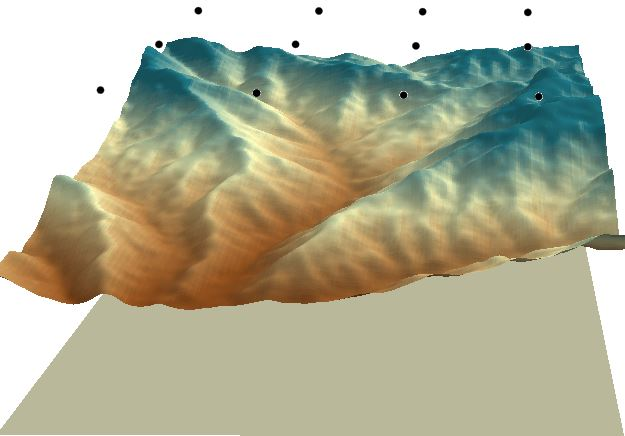
\includegraphics[width=0.8\textwidth]{INTRO.JPG}
\caption{Rejilla de centros de esfera de falla sobre la superficie digital que representa la zona de trabajo. Elaboraci\'on propia.}
\end{figure}
Es importante resaltar que, adem\'as de no estar contemplado entre los alcance ni objetivos de este proyecto, Scoops3D no posee la capacidad de simular el comportamiento de un eventual flujo de lodo o escombros desencadenado por un evento de deslizamiento o falla. 

\section{Funcionamiento de los m\'etodos de estabilidad de laderas en Scoops3D}



Como se ha mencionado anteriormente, Scoops3D se basa en la aplicaci\'on de los an\'alisis de equilibrio l\'imite por medio de los m\'etodos de de dobelas, que aplicado en un entorno tridimensional puede verse como una an\'alisis por medio de columnas.
Cada columna posee entonces lados de distancia equivalente, dados por el tama\~no de pixel que posee el DEM especificado, mientras que la altura de la columna estar\'a dada por la distancia entre la superficie del DEM y la superficie de falla.

La superficie de falla que intersecta las dobelas en profundidad es una esfera con centro en cualquier lugar sobre la superficie del DEM y un radio \textit{r}. Scoops3D incluye en el an\'alisis de cada superficie de falla todas y cada una de las columnas cuyo p\'ixel correspondiente posea 2 o mas v\'ertices al interior de la superficie de falla.\\

La superficie de falla en la base de cada columna puede discretizarse como un plano con inclinacion $ \xi$ el cual se encuentra a una distancia \textit{R} del centro de la esfera de falla.


\subsection{inclinacion del plano basal}


Partiendo de la ecuacion para la generacion de una superficie esferica:

$$ \textit{R}^{2} = \textit{x}^{2} + \textit{y}^{2} + \textit{z}^{2}$$

por lo cual el buzamiento aparente $\xi$ del plano estaria dado por
$$ \xi = \textit{cos}^{-1}  (\dfrac{1}{\sqrt{1+(\partial z/ \partial x)^{2} + (\partial z/ \partial y)^{2} }})   $$ 

mientras que el buzamiento real $ \alpha$ estaria representado por \\
$$ \alpha = tan^{-1} ((\partial z/ \partial x)\textit{cos}\varphi +(\partial z/ \partial x)\textit{sin}\varphi )  $$
donde $\varphi$ es la direccion de buzamiento de la ladera en el lugar donde se encuentra ubicada la columna

Teniendo entonces los l\'imites de la columna de an\'alisis, es posible calcular su vol\'umen, y posteriormente su peso.

\subsection{Vol\'umen de la columna}



\begin{figure}[h]
\caption{Columna de evaluaci\'on}
\centering
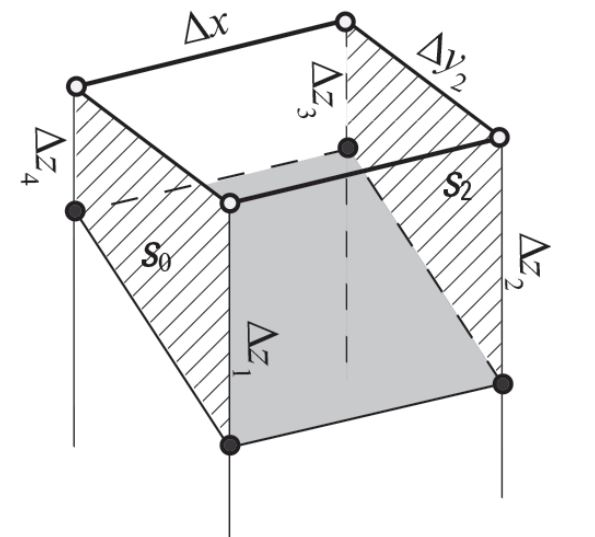
\includegraphics[width=0.5\textwidth]{complete_column.JPG}
\caption{Representaci\'on gr\'afica de una columna completamente contenida dentro de una esfera de evaluaci\'on. Fuente: Manual de usuario de Scoops3D.}
\label{fig:Interfaz de usuario}
\end{figure}

Dado que scoops3D tiene en cuenta todas aquellas columnas que contengan 2 vertices al interior de la esfera de busqueda, es posible que solo una parte de la columna este contenida dentro de dicha esfera, caso en el cual el volumen de dicha parte incluida debe ser calculado.
En este caso y partiendo de la figura 3.2, se toma un plano intermedio $ S_{1} $ entre los planos $ S_{0} $ y $ S_{2} $

En los casos en los que una columna es contenida es su totalidad, es decir, que sus planos  paralelos $S_{0}$ y $S_{2}$ tienen igual area. el volumen (\textit{V}) estara dado por 

$$\textit{V}= (1/6)\vartriangle \textit{x}(S_{0} + 4S_{1} + S_{2})$$

donde el area del plano $\textit{S}_{0}$ estara dada por
$$ \textit{S}_{0} = (1/2)(\vartriangle z_{1} +\vartriangle z_{1})+\vartriangle \textit{y}_{1}  $$

y el area del plano paralelo $\textit{S}_{0}$
$$ \textit{S}_{2} = (1/2)(\vartriangle z_{2} +\vartriangle z_{3})+\vartriangle \textit{y}_{2}  $$

Finalmente, el peso $W$ de la columna estara representado por

$$\textit{W} = \int \textit{V} \gamma (\textit{z}) \textit{dz} $$

Donde $ \gamma$ es el peso unitario del suelo, el cual puede variar con la profundidad $\textit{z}$

En general, los m\'etodos de equilibrio l\'imite definen el Factor de seguridad (F) como la relaci\'on entre las fuerzas resistentes  \textit{s} y las fuerzas actuantes $\tau$

$$F =\frac{\textit{s}}{\tau}$$

Donde F inferior a uno (1) indica inestabilidad. Para \'areas definidas, como el \'area en la base de cada columna (\textit{A})

La fuerza actuante (\textit{T}) sobre \textit{A} estar\'a dada por

$$\textit{T}=\left(\frac{1}{\textit{A}}\right)\int_{\textit{A}}^{} \frac{\textit{s}\textit{A}}{\textit{F}} \textit{dA}$$

Discretizando las componentes\textit{i} y \textit{j} correspondientes a las fuerzas resistentes \textit{x} y \textit{y} respectivamente, se tiene.

$$\textit{T} = \frac{1}{\textit{F}} \Sigma\textit{s}_{\textit{i,j}} \textit{A}_{\textit{i,j}}$$

\begin{center}


\begin{tabular}{|c|c|c|c|c|c|c|c|c|c|}
\hline 
\textit{i,j} & \textit{i,j} & \textit{i,j} & \textit{i,j} & \textit{i,j} & \textit{i,j} & \textit{i,j} & \textit{i,j} & \textit{i,j} & \textit{i,j} \\ 
\hline 
\textit{i,j}& \textit{i,j}& \textit{i,j} & \textit{i,j} &\textit{i,j} & \textit{i,j} & \textit{i,j} & \textit{i,j} & \textit{i,j} & \textit{i,j} \\ 
\hline 
\textit{i,j} & \textit{i,j} & \textit{i,j} & \textit{i,j} & \textit{i,j} & \textit{i,j} & \textit{i,j} & \textit{i,j} & \textit{i,j} & \textit{i,j} \\ 
\hline 
\textit{i,j} & \textit{i,j} & \textit{i,j} & \textit{i,j} & \textit{i,j} & \textit{i,j} & \textit{i,j} & \textit{i,j} & \textit{i,j} & \textit{i,j} \\ 
\hline 
\textit{i,j} & \textit{i,j} & \textit{i,j} & \textit{i,j} & \textit{i,j} & \textit{i,j} & \textit{i,j} & \textit{i,j} & \textit{i,j} & \textit{i,j} \\ 
\hline 
\textit{i,j}& \textit{i,j}& \textit{i,j}& \textit{i,j} & \textit{i,j}& \textit{i,j}& \textit{i,j} & \textit{i,j} &\textit{i,j} & \textit{i,j} \\ 
\hline 
\textit{i,j} &\textit{i,j} & \textit{i,j} & \textit{i,j} & \textit{i,j} & \textit{i,j}& \textit{i,j}& \textit{i,j} & \textit{i,j}& \textit{i,j} \\ 
\hline 
\textit{i,j} & \textit{i,j}& \textit{i,j}& \textit{i,j} & \textit{i,j} & \textit{i,j} & \textit{i,j} & \textit{i,j}& \textit{i,j} & \textit{i,j}\\ 
\hline 
1,2 & 2,2 & \textit{i,j} & \textit{i,j} & \textit{i,j} & \textit{i,j}& \textit{i,j} & \textit{i,j} & \textit{i,j}& \textit{i,j}\\ 
\hline 
1,1 & 2,1 & \textit{i,j}& \textit{i,j} & \textit{i,j} & \textit{i,j} & \textit{i,j} & \textit{i,j}& \textit{i,j} & \textit{i,j}\\ 
\hline 
\end{tabular} 
\end{center}
La columna $\textit{i}=1$ y $\textit{j}=1$ ser\'a aquella ubicada en la posici\'on del p\'ixel en la esquina inferior izquierda del DEM.

El equilibrio de momentos se calcula a lo largo de un eje rotacional basado en el centro de la esfera de falla, dicho eje es horizontal y normal a la direcci\'on potencial de falla.
El momento actuante est\'a direccionado principalmente por la fuerza de la gravedad (\textit{W})
$$a_{i,j}=R_{i,j}\sin \alpha_{i,j}$$ 

Donde $\textit{R}_{i,j}$ es la distancia desde el centro de la esfera hasta el centro del \'area $\textit{A}$ en la base de la columna, $\alpha_{i,j}$ es el buzamiento aparente del plano de \'area (\textit{A}) visto desde la posici\'on del centro de la esfera. En $\textit{R}_{i,j}$ se puede apreciar una de las principales diferencias entre el an\'alisis de equilibrio limite en 2D y 3D, ya que en 3D dicha distancia siempre es variable, por lo cual el momento actuante ($\textit{M}_{act}$) de cada columna debe calcularse independientemente, para lo cual se usa la expresi\'on:

$$\textit{M}_{act}=\Sigma \textit{R}_{i,j}\textit{W}_{i,j}\sin\alpha_{i,j}  $$

El momento resistente($\textit{M}_{r}$)  est\'a representado por la sumatoria de los productos de esfuerzos cortantes en la parte inferior de cada columna.

$$\textit{M}_{Total}= \Sigma \textit{R}_{i,j}\frac{\textit{s}_{i,j}\textit{A}_{i,j}}{\textit{F}}  $$
por lo que al reemplazar $\textit{s}_{i,j}$ 

$$ {M}_{Total} = \Sigma \textit{R}_{i,j} \frac{\textit{C}_{i,j}\textit{A}_{i,j}+(\textit{N}_{i,j}-\textit{U}_{i,j}\textit{A}_{i,j})\tan\phi_{i,j}}{\textit{F}} $$

Donde $\textit{N}_{i,j}$ es la fuerza normal correspondiente a cada columna.\\

El momento de equilibrio para una columna individual estar? dada entonces por la expresion.
$$ \Sigma \textit{M}= \Sigma \textit{R}_{i,j} \frac{\textit{c}_{i,j}\textit{A}_{i,j}+(\textit{N}_{i,j}-\textit{u}_{i,j}\textit{A}_{i,j})\tan\phi _{i,j}}{F}-\Sigma \textit{W}_{i,j}\textit{R}_{i,j}\sin \alpha _{i,j} $$

Por lo que el factor de seguridad \textit{F} Est\'a dado por:

$$\textit{F}_{i,j}=  \frac{\Sigma \textit{R}_{i,j}(\textit{c}_{i,j}\textit{A}_{i,j}+(\textit{N}_{i,j}-\textit{u}_{i,j}\textit{A}_{i,j})\tan \phi _{i,j}}{\Sigma \textit{W} _{i,j}(\textit{R} _{i,j}\sin\alpha _{i,j})}  $$


\section{Modelo de elevaci\'{o}n digital.}


Un modelo de elevaci\'{o}n digital (DEM por sus siglas en ingl\'{e}s) es un formato de archivo empleado para representar digitalmente una superficie, incluyendo sus variaciones e irregularidades. Para su elaboraci\o'n pueden utilizarse herramientas como fotogrametr\'ia, interferometr\'ia, radar, laser, entre otros. \cite{whatisadem}


T\'{e}rminos sin\'{o}nimos a  ``modelo de elevaci\'{o}n digital '' son Modelo digital de terreno (DTM por
sus siglas en ingl\'{e}s) y Modelo Digital de Superficie (DSM por sus siglas en ingl\'{e}s).
La informaci\'{o}n contenida en un DEM puede representarse en forma Raster (rejilla de
p\'ixeles), de forma vectorial como un TIN (Triangular Irregular Network por sus siglas en
ingl\'{e}s) o simplemente por puntos de coordenadas XYZ a partir de los cuales se puede
generar un DEM tipo RASTER o TIN. \cite{tachikawa1994development} \\
 Gracias a la capacidad de c\'{o}mputo que poseen las
herramientas SIG actuales, los DEM generados por los sensores remotos actuales cuentan
con resoluciones que alcanzar pocos cent\'imetros por pixel y abarcan importantes extensiones de la superficie terrestre. \cite{zhang2002comparison}  \cite{hirt2010comparison}
\\
\subsection{ESRI ASCII}

El modelo de superficie trabajado en este proyecto es un DEM RASTER en el formato ESRI
ASCII (extensi\'{o}n \textbf{.asc}) este archivo cuenta con el siguiente encabezado al abrirse desde un
editor de texto.

\begin{lstlisting}
  NCOLS xxx
    NROWS xxx
    XLLCENTER xxx | XLLCORNER xxx
    YLLCENTER xxx | YLLCORNER xxx
    CELLSIZE xxx
    NODATA_VALUE xxx
    row 1
    row 2
    ...
    row n
\end{lstlisting}

De este encabezado puede obtenerse el n\'{u}mero de celdas, n\'{u}mero de columnas, tama\~{n}o de celda (metros
sobre la superficie terrestre que representa cada p\'{i}xel, debe ser mayor a cero),
coordenadas x,y del origen y valor que representa la ausencia de informaci\'{o}n.
ASTER GDEM V2
La segunda versi\'{o}n de ASTER(Advanced Spaceborne Thermal Emission and Reflection
Radiometer) GDEM (Global Digital Elevation Model) fue realizada por la NASA (United
States National Aeronautics and Space Administration) y publicada el 17 de Octubre de
2011. Esta adquisici\'{o}n consta de topografia digital a escala global y comprende hasta un
99\% de la superficie terrestre, siendo esta la adquisici\'{o}n de datos topogr\'{a}ficos con mayor
extensi\'{o}n hecha p\'{u}blica hasta la fecha.
La resoluci\'{o}n m\'{a}xima de pixel en esta adquisici\'{o}n es de hasta 30m por pixel
DEM Usado.
El modelo de elevaci\'{o}n digital empleado en este trabajo corresponde a una muestra tomada
de ASTER GDEM V2 comprendida entre la coordenadas 650354.816N 8469349.749 W
641724.797 S 8457102.358 E (metros mercator).La resoluci\'{o}n de pixel obtenida para esta
zona es de 38m seg\'{u}n consta en el encabezado del DEM Arc ASCII. El sistema de
coordenadas asignado al DEM es $ MAGNA\_SIRGAS\_Colombia\_West\_zone$.\par

\begin{lstlisting}

ncols         182
nrows         151
xllcorner     1108419.546
yllcorner     1137605.366
cellsize      38.218514142587
NODATA_value  -9999
\end{lstlisting}

El DEM usado en este proyecto se muestra en la imagen \ref{fig:dem usado}
\section{Interfaz de usuario.}

A continuaci\'on se describen las herramientas disponibles  en Scoops3D empleadas en las pruebas preliminares (secci\'on \ref{chap:pruebas preliminares}) y la posterior ejecuci\'on de con datos extra\'idos de las muestras recolectadas en campo.
Esta secci\'on se ha compuesto a partir del manual de usuario de Scoops3D y de la experiencia obtenida con el uso del software.



\begin{figure}[h]
\centering
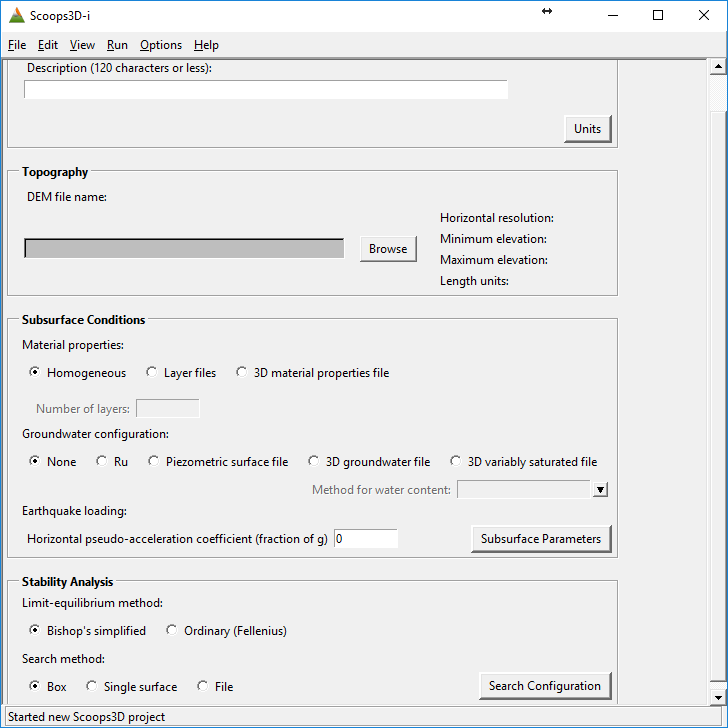
\includegraphics[width=0.5\textwidth]{main_window.PNG}
\caption{Captura de la ventana principal de Scoops3D en el sistema operativo Windows. Elavoraci\'on propia.}
\label{fig:Interfaz de usuario}
\end{figure}

La interfaz de usuario principal de Scoops3D  cuenta con 4 secciones principales tituladas Description, Topography, Subsurface Conditions y Stability Analysis. En la secci\'{o}n Description se cuenta con un recuadro de texto en el cual el usuario puede introducir una descripci\'{o}n del proyecto a realizar, adicionalmente, se cuenta con un bot\'{o}n titulado Units (unidades) cuyo funcionamiento se describe a continuaci\'{o}n. \\

\begin{figure}[H]
\centering
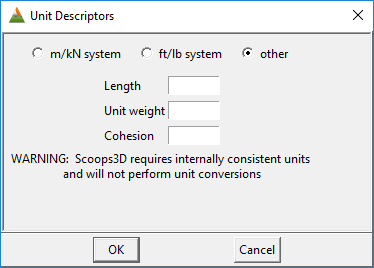
\includegraphics[width=0.5\textwidth]{units_winow.PNG}
\caption{Las unidades seleccionadas pueden modificarse posteriormente.}
\label{unidades}
\end{figure}


En la ventana de selecci\'{o}n de unidades el usuario puede seleccionar las unidades de
esfuerzo a trabajar, o trabajar en sus propias unidades personalizadas. Sin embargo, es
fundamental tener en cuenta que Scoops3D no realiza conversi\'{o}n alguna al momento de su
ejecuci\'{o}n. Por lo cual se debe tener claridad sobre las unidades longitudinales que posee el
DEM as\'{i} como las unidades de \'{a}rea ingresadas en la ventana de b\'{u}squeda de superficie de
falla. Su estructura se ilustra en la figura \ref{unidades}
\\
\begin{figure}[h]
\centering
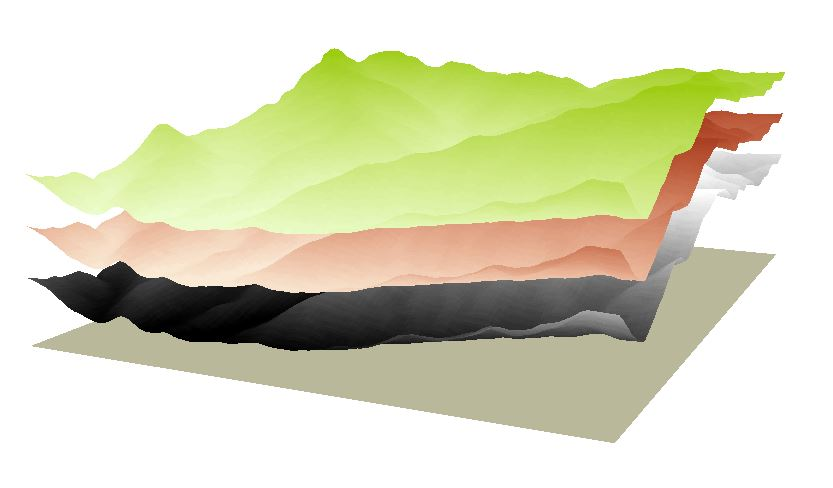
\includegraphics[width=0.9\textwidth]{model.JPG}
\caption{Representaci\'on de distintas geol\'ogicas (verde, rojo, negro). Elaboraci\'on propia.}
\label{geo-units}
\end{figure}


\textbf{Condiciones superficiales.}\\
Scoops3D posee la capacidad de integrar distintas unidades estratigr\'{a}ficas en la simulaci\'{o}n
de superficie de falla. La representaci\'{o}n geom\'{e}trica de dichas unidades se pueden ingresar
a Scoops3D por medio de DEM que representen el techo de cada unidad.
Para usar esta funcionalidad se debe marcar el checkbox layer files en la ventana principal
de Scoops3D.
\\

En caso de ser necesario el uso de varias unidades estratigr\'{a}ficas, es necesario ingresar
los par\'{a}metros de resistencia de cada una de los materiales representados, para lo cual se
hace uso de la ventana de par\'{a}metros subsuperficiales. ilustrada en la figura \ref{fig:parameters}. En esta ventana no es necesario  digital las unidades (MPa) o s\'imbolo alguno para representar los grados del par\'ametro  fi \\

\begin{figure}[H]
\centering
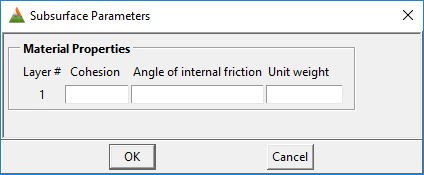
\includegraphics[width=0.8\textwidth]{material_properties_window.PNG}
\caption{Captura de la ventana de introducci\'on de p\'arametros de resistencia de unidades geol\'ogicas sup-superficiales. Elavoraci\'on propia.}
\label{fig:parameters}
\end{figure}


De la misma manera, la cabeza piezom\'{e}trica o nivel fre\'{a}tico se puede representar por
medio de un modelo de elevaci\'{o}n digital como se ilustra en la figura \ref{modelo piezometrico}
\\


\begin{figure}[H]
\centering
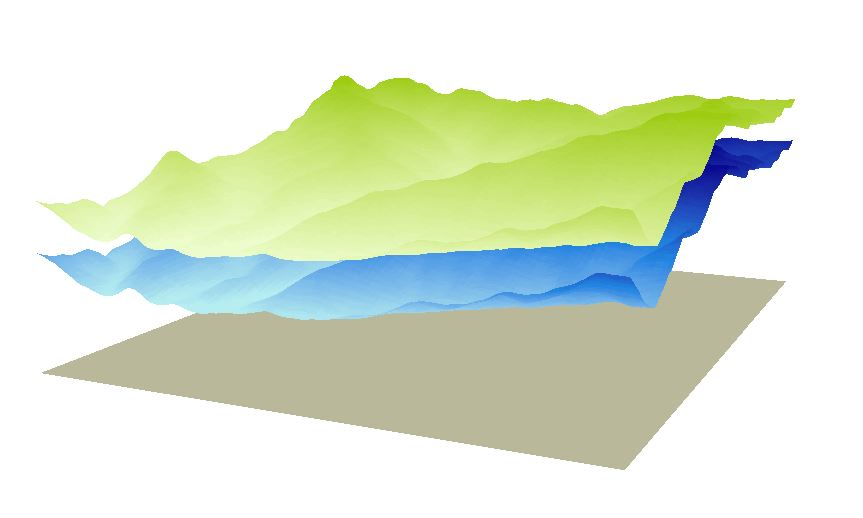
\includegraphics[width=0.8\textwidth]{piezo.JPG}
\caption{Representaci\'on de un nivel priezom\'etrico (azul) como una superficie bajo el DEM superficial (verde). Elaboraci\'on propia.}
\label{modelo piezometrico}
\end{figure}

\textbf{An\'{a}lisis de estabilidad}\\
En el apartado de an\'{a}lisis de estabilidad de la ventana principal de Scoops3D se puede
seleccionar el m\'{e}todo de an\'{a}lisis de estabilidad de laderas que se desea emplear. Las
opciones disponibles son Bishop simplificado y Fellenius.
Asimismo se puede seleccionar el m\'{e}todo de b\'{u}squeda de superficie de falla, las opciones
disponibles son caja, cuyo funcionamiento se detalla en el uso de la ventana search-box.
Superficie espec\'{i}fica, el cual eval\'{u}a la posibilidad de ocurrencia de superficies de Falla
respecto a un \'{u}nico centro de esfera determinado por el usuario. Y por \'{u}ltimo el m\'{e}todo de
b\'usqueda por medio de un archivo de coordenadas XYZ las cuales deber\'an corresponder a
los centros de esfera de falla a evaluar.\par

\textbf{M\'{e}todo de B\'{u}squeda por caja}\\
Inicialmente se definen las dimensiones de la caja de trabajo (figura \ref{searchbox-parameters}) en la cual Scoops3D buscar\'{a}
superficies de Falla. La extensi\'{o}n de dicha caja estar\'{a}n dadas por la altitud m\'{i}nima y
m\'{a}xima del DEM a trabajar y el alcance norte-sur y este-oeste del mismo,el usuario es libre
de modificar estas caracter\'{i}sticas y trabajar con una extensi\'{o}n superior o inferior a las del
DEM.
\begin{figure}[H]
\centering
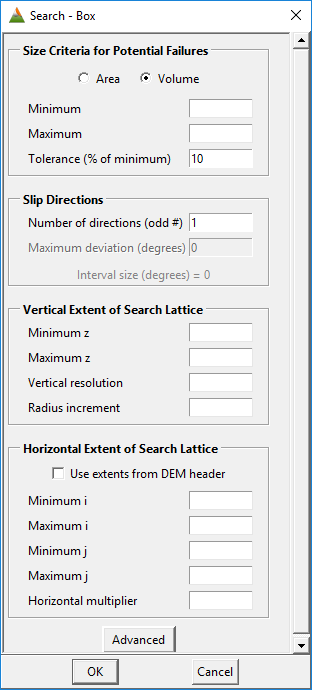
\includegraphics[scale=0.5,keepaspectratio]{search_config_window.PNG}
\caption{Ventana de par\'ametros de la caja de b\'usqueda de superficies de falla, la resoluci\'on de dicha rejilla de b\'usqueda impacta directamente en el tiempo que toma la ejecuci\'on de Scoops3D, este, al ser un programa basado en la arquitectura  bits) no obtiene mayor ventaja con el uso de altas cantidades de memoria RAM ni procesadores con elevado n\'umero de n\'ucleos}
\label{searchbox-parameters}
\end{figure}


	\section{Archivos de salida.}
\label{chap: archivos de salida}
Scoops3D tiene la capacidad de producir una gran variedad de archivos de salida los
cuales le posibilitan al usuario obtener informaci\'{o}n acerca del an\'alisis realizada as\'{i} como
obtener un estimativo de la distribuci\'{o}n espacial de los factores de seguridad para las zonas
contenidas en el DEM base, teniendo en cuenta los par\'{a}metros de resistencia introducidos.
Cada archivo de salida est\'{a} compuesto principalmente por el nombre del proyecto ejecutado, seguido por el car\'{a}cter gui\'{o}n bajo (\_) y el nombre respectivo del archivo generado.
En la siguiente tabla se listan los archivos est\'{a}ndar de salida junto con su respectiva descripci\'{o}n.


% Please add the following required packages to your document preamble:
% \usepackage{booktabs}
\begin{table}[H]
\centering
\caption{Tabla descriptiva de los archivos generados en una ejecuci\'on est\'andar de Scoops3D.}
\label{output_files}
\begin{tabular}{@{}ll@{}}
\toprule
\_out.txt          & \begin{tabular}[c]{@{}l@{}}Este archivo en formato de texto plano contiene\\   los par\'{a}metros de resistencia y par\'{a}metros de b\'{u}squeda introducidos en la\\   interfaz de usuario de Scoops3D, as\'i como informaci\'{o}n b\'asica de la prueba\\   realizada, m\'{e}todo de an\'alisis de estabilidad usado, listado de archivos de\\   salida generados, dimensiones del DEM base y DEMs generados.\end{tabular} \\ \midrule
\_fos3d\_out.asc   & \begin{tabular}[c]{@{}l@{}}Este archivo tipo ASCII DEM posee las mismas\\   dimensiones del DEM original, contiene la distribuci\'{o}n de factores de\\   seguridad calculados para cada p\'{i}xel\end{tabular}                                                                                                                                                                                             \\
\_fosvol\_out.asc  & \begin{tabular}[c]{@{}l@{}}Este archivo\\   tipo DEM contiene la magnitud de masa o metros c\'{u}bicos de material desplazado\\   en un \'{a}rea cuyo factor de seguridad sea inferior a 1\end{tabular}                                                                                                                                                                                                     \\
o                  &                                                                                                                                                                                                                                                                                                                                                                                                     \\
\_fosarea\_out.asc &                                                                                                                                                                                                                                                                                                                                                                                                     \\
\_spheres\_out.okc & \begin{tabular}[c]{@{}l@{}}Archivo DEM que expresa la ubicaci\'{o}n y altura\\   del centro de esfera de las superficies de falla encontradas y a su vez que\\   tienen factor de seguridad inferior a 1\end{tabular}                                                                                                                                                                                   \\
\_slope\_out.asc   & \begin{tabular}[c]{@{}l@{}}Este Archivo DEM es un mapa pendientes del\\   modelo de elevaci\'{o}n digital original.\end{tabular}                                                                                                                                                                                                                                                                        \\
\_errors\_out.txt  & \begin{tabular}[c]{@{}l@{}}Este archivo de texto plano contiene las\\   advertencias encontradas durante la ejecuci\'{o}n de Scoops3D. Cabe destacar que\\   la existencia de notas o errores en este archivo no implica una mala\\   ejecuci\'{o}n o mala calidad de los archivos de salida del proyecto de Scoops3D\end{tabular}                                                                          \\ \bottomrule
\end{tabular}
\label{output_table}
\end{table}


Adicionalmente se cuenta con el archivo Boundcheck. Este es un archivo raster en el cual se puede observar si los l\'mites de la rejilla de b\'usqueda ha sido una limitante para la detecci\'on de superficies de falla.
Considerando, por ejemplo, una ladera de baja pendiente compuesta por materiales de baja competencia los cuales presentan una superficie de falla ante determinadas condiciones de humedad o longitud de la ladera. En este caso,  el centro de la esfera que sigue la trayectoria de dicha superficie de falla rotacional se encontrar\'ia ubicado en una altitud considerable respecto a la ladera en cuestion.

A medida que la ladera posee una pendiente menos pronunciada, el centro de la esfera de falla tender\'ia a encontrarse en una altitud infinita.

Dado que a partir de determinados par\'ametros de resistencia la aplicaci\'on del m\'etodo de Bishop comienza a producir factores de seguridad cada vez mas elevados, no es necesario realizar pruebas en b\'usqueda de centros de esfera que se aproximen a infinito.
Sin embargo s\'i es posible realizar una b\'usqueda en la cual la altura m\'axima de centros de esfera sea una limitante para hayar superficies de falla que posean factor de seguridad  considerableente bajo. Para ello, el archivo boundcheck muestra distintos valores en funci\'on del comportamiento del centro de esfera respecto a los l\'imtes verticales y laterales de la caja de b\'usqueda.

\begin{table}[]
\centering
\caption{Representaci\'on de los valores posibles del archivo boundcheck}
\label{my-label}
\begin{tabular}{ll}
\hline
\multicolumn{1}{|l|}{\textbf{c\'odigo}} & \multicolumn{1}{l|}{\textbf{Caso encontrado}} \\ \hline
0                                     & ninguno                                           \\
100                                   & ancho m\'inimo muy alejado                          \\
900                                   & ancho m\'aximo muy cercano                          \\
10                                    & alto m\'inimo muy elevado                           \\
90                                    & alto m\'aximo muy bajo                              \\
1                                     & elevaci\'on m\'inima muy alta                         \\
9                                     & elevaci\'on m\'axima muy baja                         \\
-9999                                 & no se encontraron superficies de falla           
\end{tabular}
\label{boundcheckTable}
\end{table}

En la medida de lo posible, no se debe limitar la detecci\'on de superficies de falla a los limites vertiales y laterales de la caja de b\'usqueda empleada

\chapter{Zona de estudio.}
\label{chap_zonaEstudio}

La zona de estudio se encuentra localizada en las afueras del per\'imetro urbano del municipio de Ciudad Bol\'ivar en el Departamento de Antioquia. 
Las laderas noroxidental y suroriental de la quebrada La Linda abarcan un \'area de XX metros cuadrados con pendientes que oscilan entre el \(20\,\%\) y \(30\,\%\)
% Es importante colocar el valor del área de la ladera.
La Quebrada La Linda no posee afluente alguno, sus aguas desembocan totalmente en la quebrada La Raya.
Las pendientes m\'as pronunciadas de la cuenca hidrogr\'afica de la quebrada La Linda se encuentran aguas arribas en las cercan\'ias del Batolito Farallones, tal como se puede apreciar en la Figura \ref{fig:slopes}.

\begin{figure}[H]
\centering
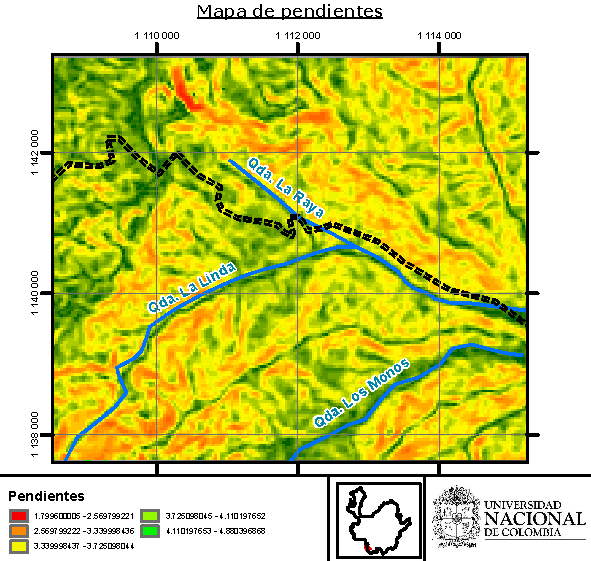
\includegraphics[scale=1]{img/pendientes.pdf}
\caption{Mapa de pendientes de la cuenca hidrogr\'afica de la quebrada La Linda y sus zonas circundantes. Elaboraci\'on propia}
\label{fig:slopes}
\end{figure}
La principal v\'ia de acceso es la carretera que desde el municipio de Ciudad B\'olivar conduce a El Carmen de Bol\'ivar.

\section{Condiciones atmosf\'{e}ricas.}
La precipitaci\'{o}n en la zona de estudio est\'{a} influenciada principalmente por la presencia de la orogenia andina, mas especificamente al flanco occidental de la cordillera occidental. La precipitaci\'{o}n anual en la zona comprendida en la plancha 165 - Carmen de Bolivar oscila entre los 5000 y 7000 mm. \cite{precipitacion} La clasificaci\'on del sector corresponde a bosque humedo premontano \cite{bosque}


\section{Geolog\'ia}
En la cuenca hidrogr\'afica de la quebrada La Linda se encuentran 3 unidades geol\'ogicas, una sedimentaria la cual corresponde al Miembro Urrao de la Fm. Penderisco y aguas arriba de la Quebrada La Linda se encuentra el Batolito Farallones.\\

\textbf{Batolito Farallones.Tmcf}
Ubicado al Sur del Stock de Cerro plateado de y de formaci\'on contemporanea a este. El Batolito Farallones recibe su nombre por encontrarse lozalizado al Este de la localidad de Farallones.
El Batolito Farallones de edad Mioceno datado por el m\'etodo $K/Ar$ como originado hace 11 +- 2 m.a. \cite{farallones}. Presenta una aureola de contacto extensa (500m aprox), fuertemente fallada y plegada con los sedimentos cret\'acicos que lo rodean en su extremo norte. Su altura alcanza apr\'oximadamente los 3400msnm exhibiendo escarpes casi totalmente verticales.
Su clasificaci\'on se determin\'o como intrusivo monzonitico.
 

\textbf{Fm. Penderisco Miembro Urrao. Ksaau}
La sedimentaci\'on de la formaci\'on penderisco se ubica entre el cretaceo temprano a tardio como producto de flujos de turbiedad.
Est\'a compuesta por estratos de rocas que var\'ian en calibre desde areniscas pasando por limolitas y lodolitas (siendo esta la facie predominante) hasta chert, este \'ultimo se presenta frecuentemente como interestratificaciones finas. Se presentan igualmente conglomerados de tama\~no de clasto altamente variable (polim\'ictico), los cuales presentan espesores y arreglos altamente variables.
Tanto algunas lodolitas como estratos de areniscas exhiben estructuras de polaridad como estratificaci\'on cruzada, 
Su estructura fue fuertemente modificada por el emplazamiento del Batolito Farallones en  Ne\'ogeno temprano. \cite{urrao}ver figura \ref{fig:mapageo}

\textbf{Fm. Barroso. Kvb}

Las rocas de esta formaci\'on abarcan una extensa variedad composicional. Desde basaltos y rocas andes\'iticas contenidas en flujos l\'avicos hasta rocas afan\'iticas. Mineralogicamente se presentan con mayor ocurrencia espilitas seguidas de diabasas, basaltos porfidicos, aglomerados y brechas.

Hacia el este de la Plancha 135 se presentan rocas masivas y frescas de coloraci\'on oscura con alto grado de deformaci\'on. Su composicion mineral\'ogica contiene clinopiroxenos y ortopiroxenos, plagioclasa, ilmenita, clorita y leucoxeno.

En la zona de trabajo se presenta en un punto aislado sobre la v\'ia que de Ciudad Bolivar conduce a Quibd\'o.
All\'i su ocurrencia se presenta en forma de diabasa altamante fracturada y de color oscuro, con intercalaciones de chert. \cite{barroso}, 




La descripci\'on geol\'ogica retomada de la informaci\'on bibliogr\'afica oficial sirvi\'o en los ensayos preliminares del software Scoops3D (secci\'on \ref{chap:pruebas preliminares}) como referencia para seleccionar los par\'ametros de resistencia a usar en dichos ensayos.

\begin{figure}[H]
\centering
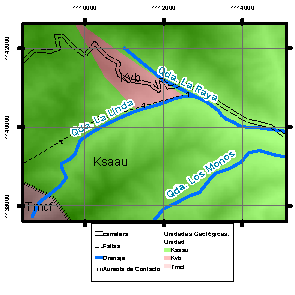
\includegraphics[scale=0.5]{img/geologia.pdf}
\caption{Mapa geol\'ogico de la zona de estudio basado en \cite{geol}. Se marca la ruta realizada durante la salida de campo y las estaciones de donde se tomaron las muestras para ensayos de laboratorio   }
\label{fig:mapageo}
\end{figure}



\section{Geomorfolog\'{i}a.}
La geomorfolog\'{i}a de la zona de estudio se presenta en la figura \ref{fig:mapageomorfo}, est\'{a} caracterizada principalmente por laderas con 23\% de pendiente con desviaci\'{o}n est\'{a}ndar del 10\%.
En la zona presenta una fuerte influencia estructural lo cual se refleja en abundante fallamiento y plegamiento, de ah\'i que la expresi\'{o}n morfol\'{o}gica de la zona exhiba laderas de pendiente media a larga con pendientes de inclinaci\'{o}n abrupta. En la Ladera norte de la Qda. La Linda se presenta un patr\'{o}n de drenaje subdendr\'{i}tico, por lo cual se clasifica esta unidad como un Gancho de Inflexi\'{o}n (Sgf), mientras que en la ladera sur el patr\'{o}n de drenaje es Subparalelo, por lo cual la unidad se caracteriza como un Espol\'{o}n Moderado de longitud larga (Sesml).  \\
Ambas laderas muestran cicatrices de movimientos en masa tipo rotacional, adicionalmente se presentan movimientos tipo traslacional en el Sesml.\cite{urrao} 
 \par


\begin{figure}[H]
\centering

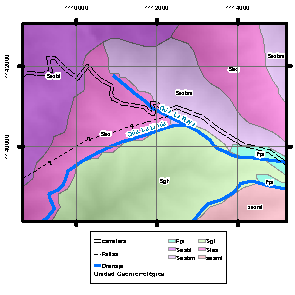
\includegraphics[width=.8\textwidth]{img/geomorfo.pdf}
\caption{Mapa geomorfol\'{o}gico de la zona de estudio. Basado en Mapa Geomorfol\'{o}gico Aplicado a Movimientos en Masa Plancha 165 El Carmen. Acercamiento.}

\label{fig:mapageomorfo}
\end{figure}
\chapter{Scoops3D.}
Tanto las pruebas prelominares como la corrida final de Scoops3D se realizaron en un equipo de
computo usando el sistema operativo Windows 10 Pro con las siguientes caracter\'{i}sticas.
Modelo MSI Procesador Intel Core i7 6700HQ. 8GB de memoria RAM DDR4, GPU Nvidia
GeForce 940mx.

\section{Prueba piloto} 

Las pruebas piloto en Scoops3D se realizaron desde la concepci\'on de este proyecto y
estuvieron encaminadas a brindar informaci\'on sobre los siguientes conceptos.



\begin{itemize}
\item Preparar la informaci\'{\o}n geogr\'{a}fica a las necesidades de funcionamiento de
Scoops3D
 \item Evaluar la calidad del DEM a usar como insumo base en Scoops3D

 \item Adquirir familiaridad con la interfaz gr\'{a}fica de usuario de Scoops3D para lograr una mejor documentaci\'on de su forma de uso.
 \item Conocer el formato de entrada de los par\'{a}metros de resistencia en la interfaz de
usuario de Scoops3D.
 \item determinar la extensi\'{\o}n espacial y resoluci\'{\o}n de la rejilla de b\'{u}squeda de superficie de falla en Scoops3D.
 \item Optimizar los par\'{a}metros de b\'{u}squeda de superficies de falla para reducir tiempo de
c\'omputo.
 \item Comprender y correlacionar los distintos archivos de salida de informaci\'{\o}n que
proporciona Scoops3D.

\end{itemize}

Durante este proceso ha sido de vital importancia contar con conocimientos en Sistemas de Informaci\'on Geogr\'afica para preparar adecuadamente los archivos de entrada, as\'i como para interpretar los archivos de salida.
\subsection{DEM usado en pruebas preliminares}

\begin{figure}[H]
\centering
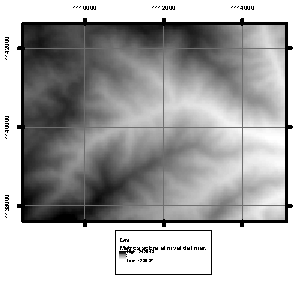
\includegraphics[scale=3]{dem.pdf}
\caption{Imagen monocrom\'atica del DEM trabajado desplegado en escala de grises. Altura m\'inima 1239 msnm, altura m\'axima 2425msnm. Elaboraci\'on propia.}
\label{fig:dem usado}
\end{figure}


Para las pruebas iniciales se us\'o el DEM mencionado en el numeral xxxxx de ASTER
GDEM V2 dada su f\'acil y r\'{a}pida adquisici\'on por medio del software Global Mapper
desarrollado por Blue Marvel.
El software Global Mapper tiene la capacidad de exportar el formato ESRI ASCII que utiliza
Scoops3D como insumo base, se recomienda exportar el DEM con la mayor resoluci\'{\o}n
posible, en caso de requerir agilizar el tiempo de procesamiento en Scoops3D, se
recomienda disminuir resoluci\'{\o}n espacial al DEM. Lo cual se puede lograr f\'{a}cilmente con la
herramienta Resample de ArcGIS en sus versiones 10 y superior (
Tool Geoprocessing
toolboxes $ (\setminus system toolboxes \setminus data management tools.tbx \setminus raster \setminus raster processing \setminus resample)$ y posteriormente la
herramienta \textbf{Raster to ASCII} $(toolboxes \setminus system toolboxes \setminus conversion tools.tbx \setminus from raster \setminus raster to ascii)$ en el software Qgis con la
herramienta Raster Calculator.\\
Debido a que Scoops3D no acepta sistemas de coordenadas geogr\'{a}ficas sino proyectadas,
se trabaj\'{\o} con el sistema de coordenadas MAGNA SIRGAS Colombia West zone. 
Se pudo comprobar que el idioma y la configuraci\'{\o}n regional puede causar que el archivo
DEM base pueda no ser compatible con Scoops3D debido al formato de separaci\'{\o}n de
decimales y unidades de miles. A continuaci\'{\o}n se muestra un archivo DEM incompatible y
uno compatible con Scoops 3D.

\begin{verbatim}
	   ncols 2
	   nrows 2
	   xllcorner 0
	   yllcorner 0
	   cellsize 1
	   NODATA_value -9999
	   0,5 1,5
	   2,5 -9999
\end{verbatim}

N\'{o}tese que la separaci\'{o}n de decimales se realiza con el car\'{a}cter coma (,). Esto como
resultado de la configuraci\'{o}n por defecto del sistema operativo Windows 10 en regiones
como am\'{e}rica latina y espa\~na.
Al introducir un archivo DEM con el formato anteriormente ejemplificado en Scoops3D, se
obtiene el siguiente error.


\newpage
\begin{verbatim}
	   ncols 2
	   nrows 2
	   xllcorner 0
	   yllcorner 0
	   cellsize 1
	   NODATA_value -9999
	   0.5 1.5
	   2.5 -9999
\end{verbatim}


El formato adecuado de DEM para usar con Scoops3D debe ser con separaci\'{o}n de
decimales con punto (.)
Finalmente se decidi\'{o} trabajar con un DEM de tama\~no de pixel 38m$\times$38m, esta es
resoluci\'{o}n obtenida de ASTER GDEM V2 sin modificaci\'on alguna para la zona de trabajo en el municipio de Ciudad Bol\'{i}var.
Este R\'aster se compone de 27.482 p\'ixeles, cubre en total \textbf{104.4 } hect\'areas,
comprende alturas entre los 1293 y los 2425 msnm.
En la zona de trabajo, con base en la informaci\'{o}n trabajada, se cuenta con laderas cuyas
pendientes alcanzan el 43 \%.

Dado que no se est\'a realizando el an\'alisis de una localidad especifica sino un \'area considerable, no se ha considerado necesario trabajar con cartograf\'ia de detalle. A manera de ensayo, se realiz\'o una corrida, con la misma extension del DEM mostrado en la figura \ref{fig:dem usado} y la misma configuraci\'on ilustrada en la figura \ref{fig:parameters}, empleando un DEM de tama\~no de pixel de 5x5 metros.
Bajo esta configuraci\'on la ejecuci\'on de Scoops3D se prolong\'o durante 30 horas sin obtener un resultado final.
\subsection{Pruebas Ejecutadas.}
En la siguiente captura de pantalla se muestran los par\'{a}metros del la caja de b\'{u}squeda
empleados en las pruebas realizadas con Scoops3D.\\

\begin{figure}[H]
\centering
	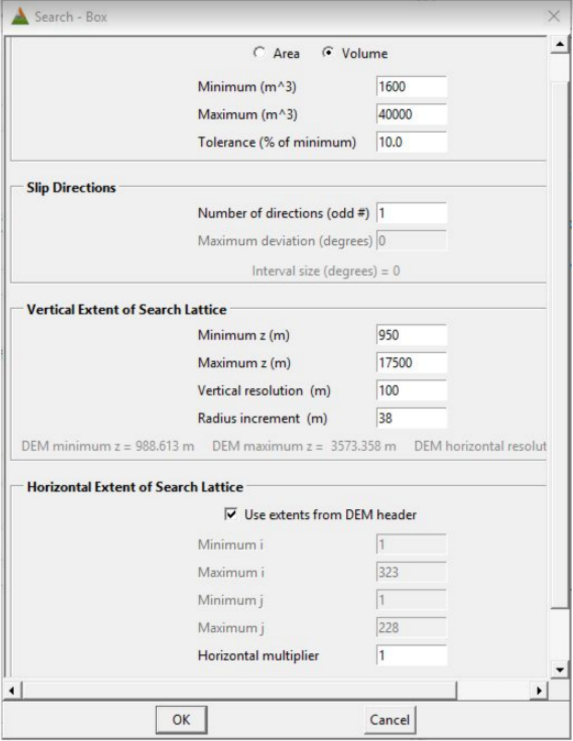
\includegraphics[scale=0.6]{search_setup.PNG} 
	\caption{Par\'ametros usados en la ejecuci\'on de pruebas preliminares.}
	\label{fig:test}
\end{figure}


Se trabaj\'{o} con el rango de b\'{u}squeda de movimientos en masa por rango de vol\'umen,
basado en los movimientos registrados en la base de datos SIMA para la zona de trabajo.
Para cada nodo de b\'{u}squeda se analiza solamente una direcci\'{o}n de deslizamiento.
En la extensi\'{o}n vertical de las dovelas de falla se toma una altura ligeramente inferior a la
altura menor existente en el DEM y como altura m\'{a}xima se tom\'{o} una altura de 17500
msnm,esta \'{u}ltima se determin\'{o} luego de m\'{u}ltiples pruebas variando la altura m\'{a}xima hasta
que se pudo apreciar que no se detectaban nuevas superficies de falla(de \'area significativa) al continuar
aumentando la altura m\'{a}xima del nodo central, para lo cual se us\'{o} el archivo Boundcheck, de acuerdo con las recomendaciones contenidas en el manual de Scoops3D. Una ilustraci\'on del archivo Boundcheck de la prueba realizada con par\'ametros de resistencia menos competentes se muestra en la figura \ref{fig:boundcheck} 

\begin{figure}[H]
\centering
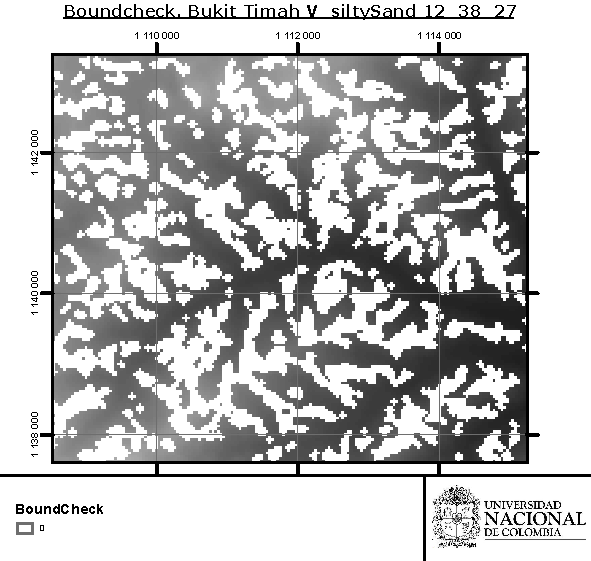
\includegraphics[scale=1]{img/boundcheck.pdf}
\caption{Mapa de distribuciones del factor Boundcheck mencionado en la secci\'on \ref{chap: archivos de salida}.
N\'otese que en su totalidad, el archivo raster Boundcheck est\'a compuesto por valores 0 (blanco) y -9999 (transparente) }
\label{fig:boundcheck}
\end{figure}




\begin{wrapfigure}{l}{0.1\textwidth} %this figure will be at the right
    \centering
    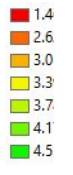
\includegraphics[scale=0.7]{symbology.PNG}
\end{wrapfigure}


Se ha implementado una escala de calor para los valores de factor de seguridad a los
pixeles de los archivos fos3D\textunderscore out.asc, aunque se han obtenido factores de seguridad hasta
un valor de 100, a los p\'ixeles con valor superior a 5 se les ha asignado la misma tonalidad
de verde.
\\


\subsection{Par\'ametros de resistencia.}
Los proyectos se han nombrado en funci\'{o}n de los par\'{a}metros de resistencia usados,
separados por el car\'{a}cter gui\'{o}n bajo y sin incluir decimales, por ejemplo 14\_45\_26\\

Los par\'ametros de resistencia para las pruebas preliminares se han seleccionado con base en las caracter\'isticas geol\'ogicas descritas para el Miembro Urrao de la Fm. Penderisco y  de los diarios de campo descargados de la base de datos SIMMA \cite{libreta}

En \cite{singapore} ademas de presentar similitud en las condiciones geol\'ogicas de la cuenca hidrogr\'afica de la quebrada la linda, tambi\'en se describen condiciones atmosf\'ericas similares a las del \'area de estudio, como precipitaciones anuales entre 2000mm y 3000mm, humedad realtiva de 84\% y temperatura promedio de 26 grados centigrados.
\linebreak 
En dicha referencia se muestran los parametros de resistencia obtenidos de muestras obtenidas a partir de n\'ucleos de perforaci\'on extraidos de la formaci\'on Bukit Timah (gran\'itica) y Jurong (sedimentaria). En ambas formaciones se han analizado varias muestras pertenecientes a distintos horizontes de meteorizacion separados de acuerdo a la denominacion de Little 1969.

Adicionalmente se han realizado pruebas con par\'ametros correspondientes a Areniscas y Limolitas descas de formaciones etandarizadas como La Fm.Pottsville(Maryland, West Virginia, Ohio. EEUU) y Fm. Repetto (South California .EEUU) 

Las muestras tomadas como referencia son: 



\begin{table}[H]
\centering
\label{tabla_parametros}
\begin{tabular}{lllll}
                                                  & Denominaci\'on de la muestra          & c   & phi & gamma                     \\ \cline{2-5} 
\multicolumn{1}{l|}{\multirow{2}{*}{Control}}     & Arenisca Pottsville                 & 14  & 45  & \multicolumn{1}{l|}{2.6}  \\
\multicolumn{1}{l|}{}                             & Limolita Repetto                    & 34  & 32  & \multicolumn{1}{l|}{2.34} \\ \hline
\multicolumn{1}{l|}{\multirow{3}{*}{Fm. Bukit Timah}} & Limo arenoso grado VI               & 26  & 27  & \multicolumn{1}{l|}{2.55} \\
\multicolumn{1}{l|}{}                             & Arena limosa grado V                & 13  & 35  & \multicolumn{1}{l|}{2.66} \\
\multicolumn{1}{l|}{}                             & Arena limosa grado V (mas profunda) & 12  & 38  & \multicolumn{1}{l|}{2.78} \\ \hline
\multicolumn{1}{l|}{\multirow{4}{*}{Fm. Jurong}}      & Arena limosa Morada                 & 125 & 42  & \multicolumn{1}{l|}{2.65} \\
\multicolumn{1}{l|}{}                             & Arena limosa Morada                 & 55  & 51  & \multicolumn{1}{l|}{2.7}  \\
\multicolumn{1}{l|}{}                             & Arena limosa Naranja                & 35  & 45  & \multicolumn{1}{l|}{2.7}  \\
\multicolumn{1}{l|}{}                             & Arena limosa Morada                 & 225 & 50  & \multicolumn{1}{l|}{2.75} \\ \cline{2-5} 

\end{tabular}
\caption{Par\'ametros de resistencia empleados en pruebas preliminares. Tomado de \cite{singapore}}
\label{tab:testtParameter}
\end{table}



\subsection{Pruebas Preliminares.}
\label{chap:pruebas preliminares}
\subsubsection{Par\'ametros de control.}

A manera de control, 2 de las corridas preliminares se realizaron empleando los par\'ametros correspondientes a rocas sanas, es decir a la arenisca de la FM. Pottsville y Limolita de la Fm. Repetto. Los DEM resultantes se muestran en las figuras \ref{fig:pottsville} y \ref{fig:repetto}.
Asimismo, entre los archivos de texto producto de ambas corridas, espec\'ificamente el archivo \_out.txt. se puede observar\linebreak


\pagebreak
\begin{center}
\textbf{siltySand\_12\_38\_27\_out.txt}

\begin{verbatim}
3D POTENTIAL FAILURE - GLOBAL MINIMUM
Bishop's 3D factor of safety:                                          15.1517
Ordinary 3D factor of safety:                                          15.1517
Volume (m ^3):                                                     3.33350E+04
Horizontal surface area (m ^2):                                    5.78697E+03
Slip surface area (m ^2):                                          5.80648E+03
Weight (kg):                                                       8.66710E+05
\end{verbatim}
\end{center}

\begin{center}

\textbf{34\_32\_23\_out.txt}
\begin{verbatim}
3D POTENTIAL FAILURE - GLOBAL MINIMUM
Bishop's 3D factor of safety:                                          12.2276
Ordinary 3D factor of safety:                                          12.2276
Volume (m ^3):                                                     3.33350E+04
Horizontal surface area (m ^2):                                    5.78697E+03
Slip surface area (m ^2):                                          5.80648E+03
Weight (kg):                                                       7.66705E+05
\end{verbatim}

\end{center}
N\'otese adem\'as que los factores de seguridad m\'iinimos son 15.15 y 12.22 para los ensayos realizados con los par\'ametros de la Fm. Repetto y Fm. Pottsville respectivamente, y las masas de material removido son de $8.66^{5}$ Kg y $7.66^{5}$Kg

\subsubsection{Par\'ametros de prueba: Fm. Bukit Timah.}
\begin{figure}[H]
\centering
\begin{minipage}{.45\linewidth}
  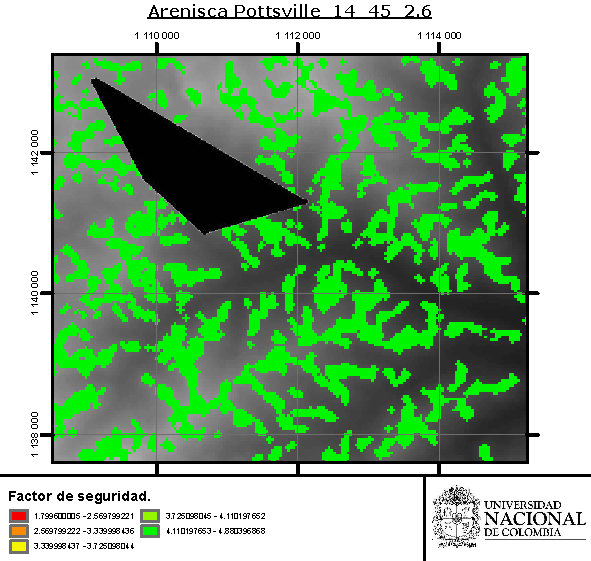
\includegraphics[width=\linewidth]{AreniscaPottsville.pdf}
  \captionof{figure}{Simulaci\'on con par\'ametros tomado de la arenisca de Fm. Pottsville.}
  \label{fig:pottsville}
\end{minipage}
\hspace{.05\linewidth}
\begin{minipage}{.45\linewidth}
  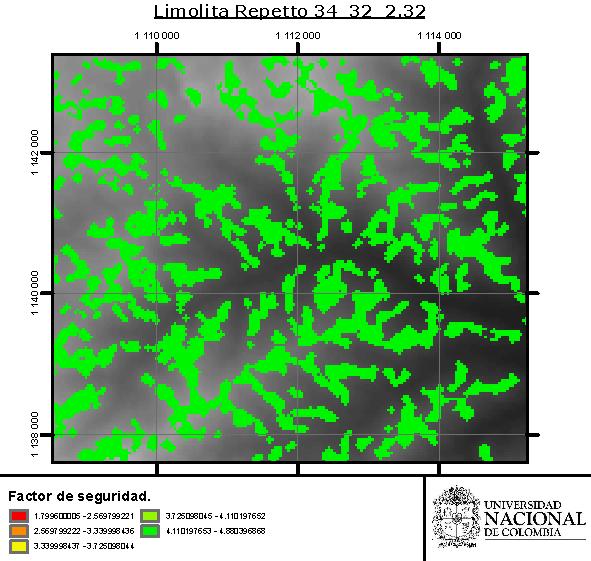
\includegraphics[width=\linewidth]{img/LimolitaRepetto34_32_232.pdf}
  \captionof{figure}{Simulaci\'on con par\'ametros tomado de la limolita de Fm. Repetto.}
  \label{fig:repetto}
\end{minipage}
\end{figure}

Al usar los par\'metros correspondientes a los distintos niveles de meteorizaci\'on de la formaci\'on Bukit Timah, se puede apreciar que a medida que se incrementa el nivel de clasificaci\'on, mayores extensiones de \'area muestran reducci\'on en el factor de seguridad.
Se aprecia igualmente que los fondos de los valles as\'i como los filos de las laderas no exhiben ocurrencia de superficies de falla, ello debido a la disminuci\'on en las pendientes existentes, aun cuando se ha buscado centros de esfera a alturas superiores a los 17.000 msnm.


\subsubsection{Par\'ametros de prueba: Fm. Jurong.}

\begin{figure}[H]
\centering
\begin{minipage}{.45\linewidth}
  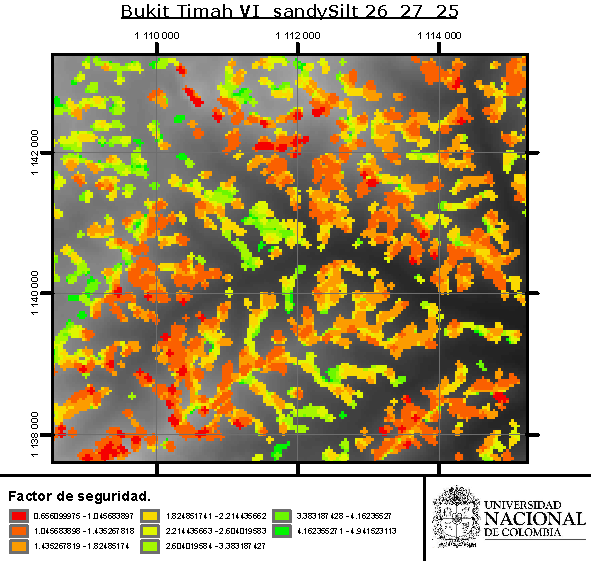
\includegraphics[width=\linewidth]{Bukit_Timah_VI_sandySilt_26_27_25.pdf}
  \captionof{figure}{}
  \label{fig:bukit1}
\end{minipage}
\hspace{.05\linewidth}
\begin{minipage}{.45\linewidth}
  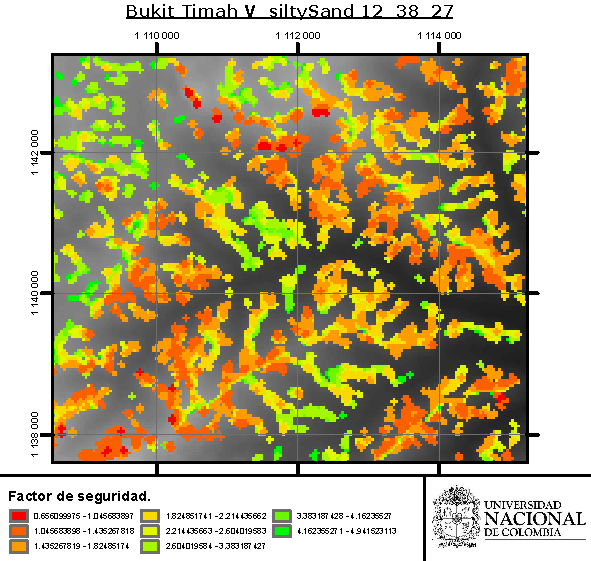
\includegraphics[width=\linewidth]{Bukit_Timah_V_siltySand_12_38_27.pdf}
  \captionof{figure}{}
  \label{fig:bukit2}
\end{minipage}
\begin{minipage}{.45\linewidth}
  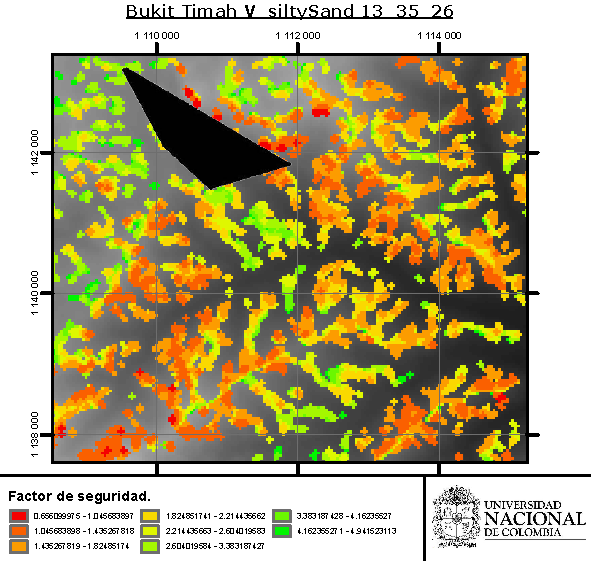
\includegraphics[width=\linewidth]{BukitTimahV_siltySand13_35_26.pdf}
  \captionof{figure}{}
  \label{fig:bukit3}
\end{minipage}
\end{figure}




Simulaciones con Par\'metros de la Fm. Jurong.


\begin{figure}[H]
\centering
\begin{minipage}{.45\linewidth}
  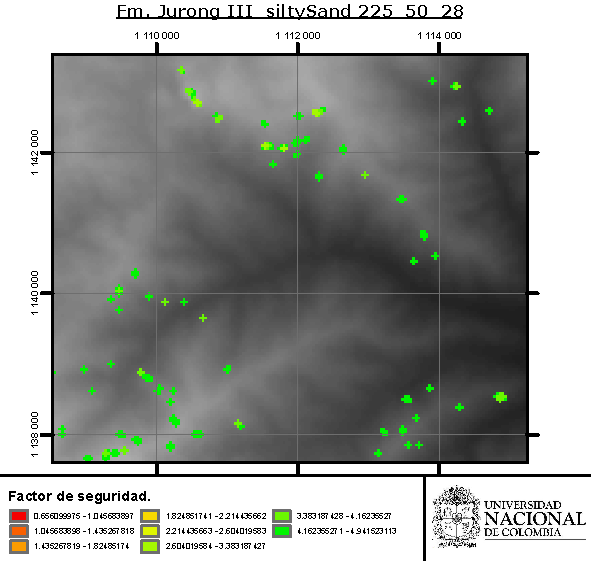
\includegraphics[width=\linewidth]{Fm_JurongIII_siltySand225_50_28.pdf}
  \captionof{figure}{}
  \label{fig:jurong1}
\end{minipage}
\hspace{.05\linewidth}
\begin{minipage}{.45\linewidth}
  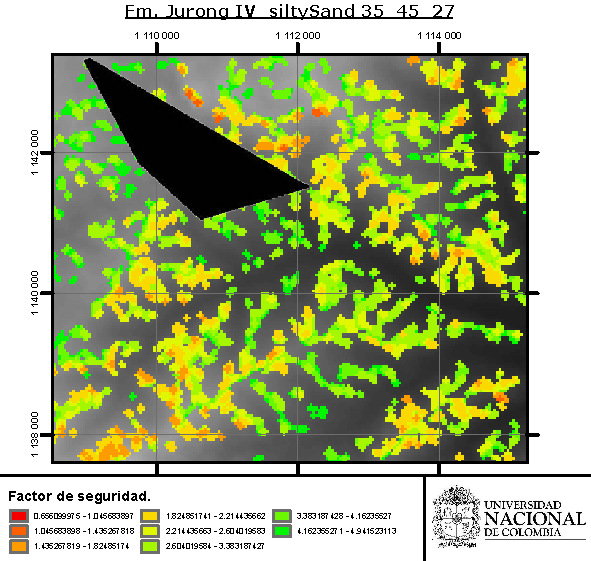
\includegraphics[width=\linewidth]{Fm_JurongIV_siltySand35_45_27.pdf}
  \captionof{figure}{}
  \label{fig:jurong2}
\end{minipage}
\begin{minipage}{.45\linewidth}
  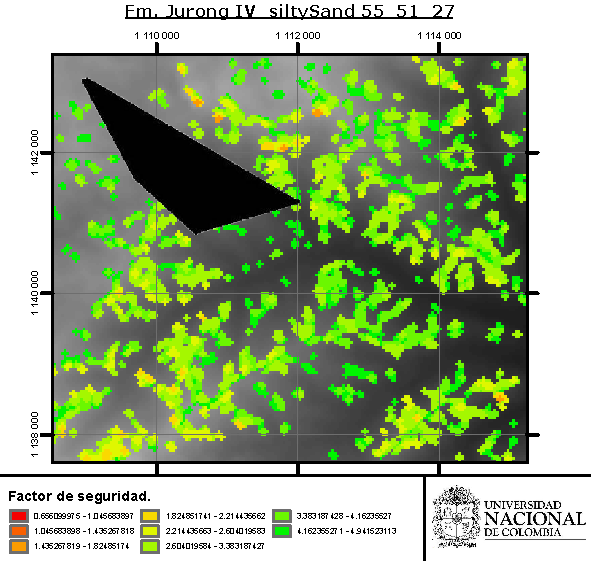
\includegraphics[width=\linewidth]{Fm_JurongIV_siltySand55_51_27.pdf}
  \captionof{figure}{}
  \label{fig:jurong3}
\end{minipage}
\begin{minipage}{.45\linewidth}
  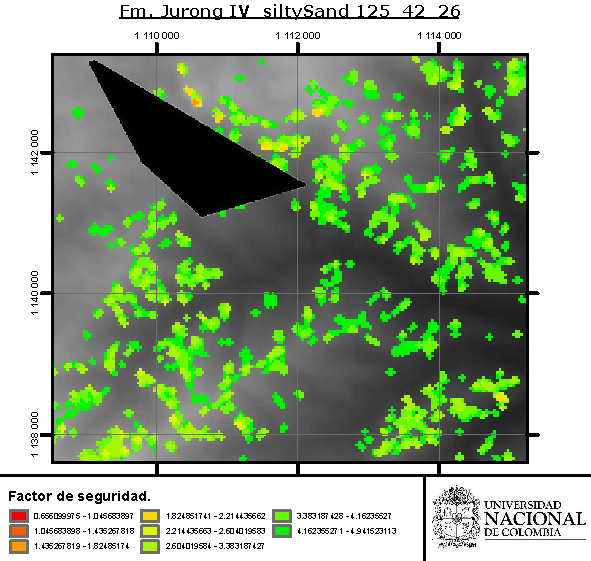
\includegraphics[width=\linewidth]{Fm_JurongIV_siltySand125_42_26.pdf}
  \captionof{figure}{}
  \label{fig:jurong4}
\end{minipage}
\end{figure}


Se puede apreciar que en las pruebas realizadas con par\'ametros correspondientes a muestras m\'s superficiales, la dispersi\'on de colores rojizos y anaranjados es mas predominante sobre la zona  de trabajo. Ello indicando una disminuci\'on en los factores de seguridad en las laderas de la zona de estudio.\par

\subsection{Interpretacion}
Es posible es posible apreciar, basado en los resultados obtenidos en la Subsecci\'on \ref{chap:pruebas preliminares} que debido a la alta variabilidad de pendientes que se presentan en la zona de trabajo, las cuales var\'ian desde bajas hasta altas y muy altas, sumado a la importante longitud de las laderas . Que el rango de factores de seguridad obtenidos con el software Scoops3D var\'ia desde valores inferiores a 1 que implican falla, hasta valores que tienen como resultado factores de seguridad superiores a 5.
Es importante tener en cuenta que esta simulaci\'on no contempla factores externos como la sobrecarga de la cobertura vegetal ni la actividad antr\'opica, que se da fuertemente en la zona y cuya presencia puede implicar la existencia en la zona de agentes qu\'imicos que debiliten la agregaci\'on de particulas y contribuya en una potencial disminuci\'on de la cohesi\'on de los materiales.

Asimismo se puede apreciar que a medida que las pruebas realizadas con materiales que indican un estado mas avanzado del proceso de meteorizaci\'on, y por ende poseen una mayor proporci\'on de fraccion arcillosa y \'oxidos e hidr\'oxidos de hierro y aluminio, tienen como resultado una marcada disminuci\'on en los factores de seguridad. Tal como se puede apreciar al compararlas im\'agenes \ref{fig:jurong3} o \ref{fig:jurong4} de las pruebas realizadas con los par\'ametros de resistencia de la Fm. Jurong.

Basado en el origen y tipo de materiales presentes en la cuenca hidrogr\'afica de la Qda.La Linda, se esperaria que los parametros de resistencia hayados en campo se aproximen considerablemente a los usados para la simulacion ilustrada en las figuras \ref{fig:jurong2} o \ref{fig:jurong3}.  




\chapter{Informaci\'on de campo.}

\section{Recorrido de campo}

El recorrido de campo se realiz\'o entre los d\'ias 22 y 24 de noviembre de 2017. La zona recorrida se tuvo como prop\'osito divisar y en lo posible muestrear aquellos lugares que mostraron menor factor de seguridad en las pruebas preliminares y apreciar el estado de las unidades geol\'ogicas que muestra la cartograf\'ia estudiada.

En campo se pudo corroborar la consistencia de la unidad geol\'ogica predominante \(\mathsf{K_{saau}}\) (limolita), dicho material se pudo apreciar en todo el recorrido, con leve variaci\'on en su grado de meteorizaci\'on, principalmente en zonas de abundante vegetaci\'on. La morfolog\'ia abrupta de las laderas permiti\'o apreciar abundantes cicatrices de anteriores desprendimientos de material, principalmente en sectores de alta pendiente y en el trazado de la carretera que une las poblaciones de La Mansa hacia Quibd\'o en el departamento de Choc\'o.

\begin{figure}[H]
  \centering
  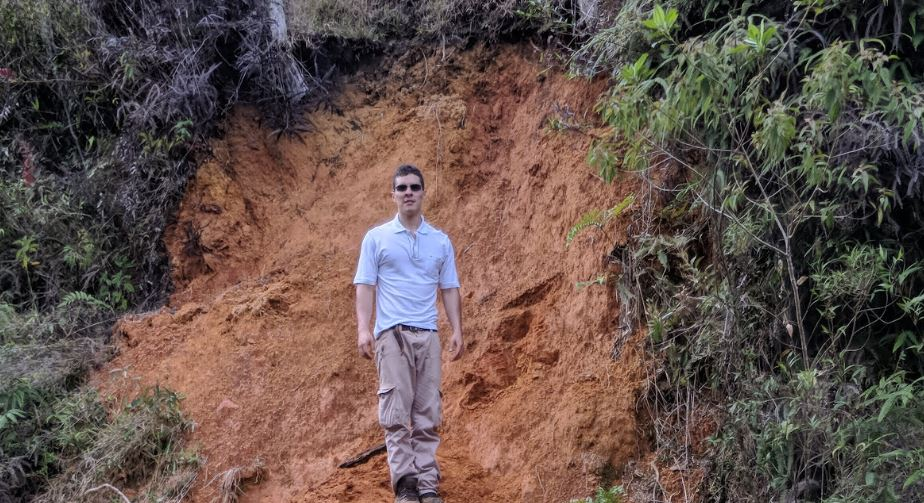
\includegraphics[scale=0.75]{img/estacion10.jpg}
  \caption{Lugar de toma de muestra de la estaci\'on 1. Aqu\'i se descartaron las zonas con material inalterado para toma de muestra en tubos PVC. Dichas muestras se tomaron donde se pod\'ia observar que el suelo conservaba su estructura original. }
  \label{fig:afloramiento}
\end{figure}

Se trabaj\'o en dos estaciones, en cada una de las cuales se realiz\'o la respectiva toma de muestra, siendo la primera de ellas la que m\'as informaci\'on proveer\'ia en los posteriores ensayos de laboratorio. Para la toma de muestra se tuvo la precauci\'on de seleccionar un lugar que no presentase retrabajamiento del material y en el cual se pudiese observar que el suelo presentase unas condiciones representativas del material observado durante los recorridos realizados.
Las muestras tomadas en la segunda estaci\'on se tomaron a una profundidad m\'a s somera (no mayor al metro) con la intenci\'on de posteriormente obtener los par\'ametros de resistencia de instancias m\'as avanzadas de meteorizaci\'on de la limonita. Esto dado que las cicatrices de movimientos en masa observadas aparentaban que aquellos eventos ocurridos se dieron hace un tiempo considerable (a juzgar por el crecimiento nueva cobertura vegetal). Asimismo, el testimonio obtenido de una habitante del lugar, corrobora que no son frecuentes movimientos que comprendan altos vol\'umenes de material, habiendo ocurrido el \'ultimo aproximadamente cinco a\~nos antes de la visita de campo.

La estaci\'on primera se realiz\'o en las coordenadas \(5.8712778, -76.0848778\), mientras que la estaci\'on segunda se realiz\'o en las las coordenadas \(5.8612472,-76.0927833\).
A continuaci\'on se detalla la informac\'on de ambas estaciones.

\textbf{Muestras recolectadas}

De la estaci\'on 1 se obtuvo:
\begin{itemize}
  \item muestra al interior de cuatro tubos PVC de \(2"\) de di\'ametro y apr\'oximadamente \(15\,\text{cm}\) de alto;
  \item un bloque de muestra inalterada  de apr\'oximadamente \(40 \times 40 \times 30\)[cm\(^3\)];
  \item una masa de \(200\,\text{g}\) de muestra alterada.
\end{itemize}

De la estaci\'on 2 se obtuvo:
\begin{itemize}
  \item Muestra al interior de 3 tubos PVC de \(2"\) de di\'ametro y apr\'oximadamente \(15\,\text{cm}\) de alto.
\end{itemize}

\begin{figure}[H]+
\centering
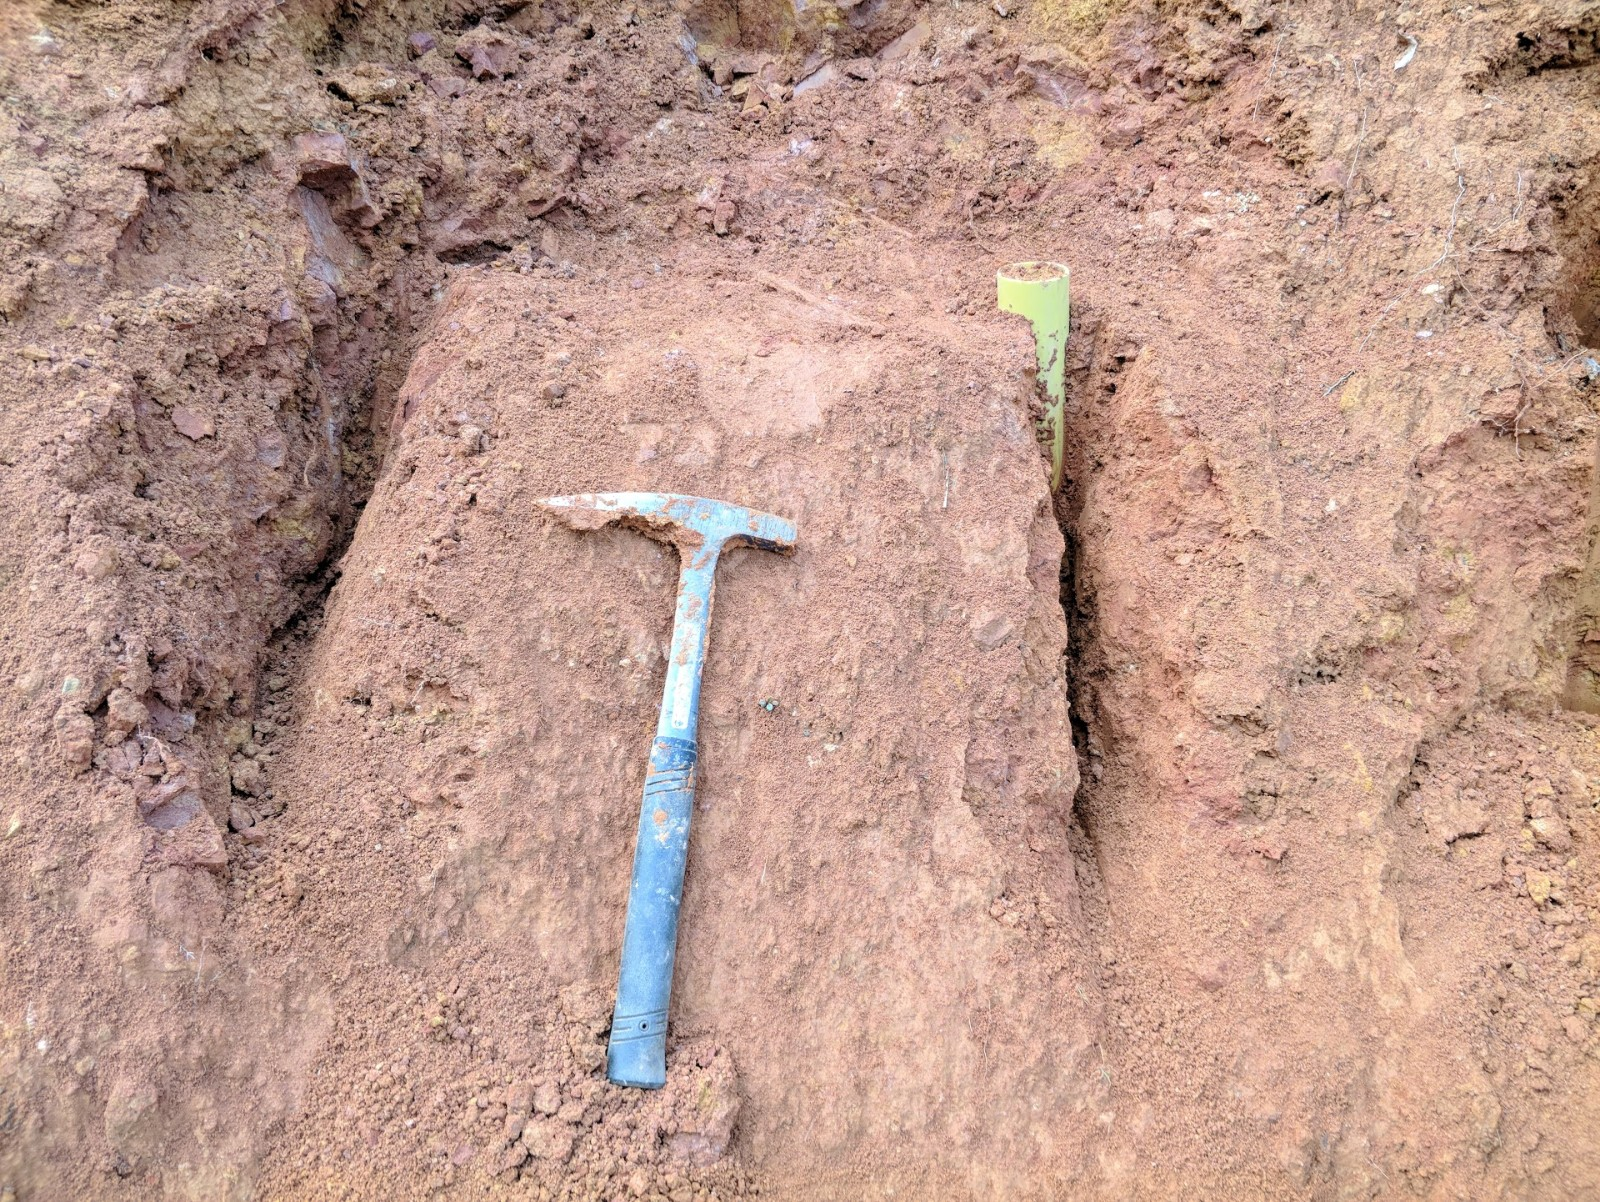
\includegraphics[scale=0.20]{img/estacion11.jpg}
\caption{Momento de toma de muestra inalterada, se tom\'o muestra en bloque as\'i como muestra confinada en tubos PCV de dos pulgadas.}
\label{fig:toma-bloque}
\end{figure}

\section{Ensayos de laboratorio.}

Las muestras recolectadas fueron analizadas en el laboratorio de suelos de a Universidad Nacional de Colombia, sede Medell\'in.
Como resultado de los ensayos se pudo determinar una humedad natural del \(21\,\%\).
La gravedad espec\'ifica de los s\'olidos, seg\'un el procedimiento descrito en la norma ASTM C-127 fue de \(2.53\).
Con estos valores se procedi\'o a realizar los ensayos de corte directo seg\'un la norma ASTM D-380. Se decidi\'o realizar los ensayos bajo condiciones de suelo saturado, es decir, habiendo sumergido totalmente la muestra de suelo durante un periodo de 24 horas, lo anterior con el prop\'osito de obtener par\'ametros correspondientes a eventos de alta precipitaci\'on que puedan presentarse en la zona de trabajo.

\begin{figure}[H]
\centering
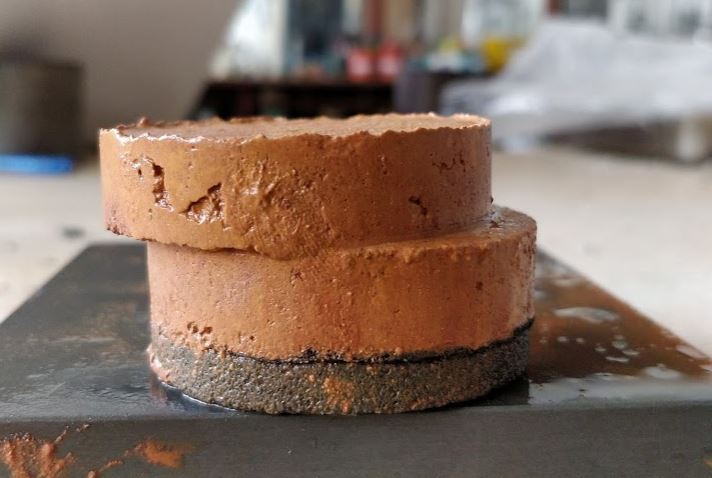
\includegraphics[scale=1]{img/fallada.jpg}
\caption{Muestra de la estaci\'on 1 en su estado posterior al ensayo de corte directo.  Desplazamiento total 6.6 mm}
\label{fig:toma-bloque}
\end{figure}


\begin{table}[H]
\centering
\caption{Caracter\'isticas f\'isicas de las muestras sometidas al ensayo de corte directo. }
\begin{tabular}{l|l|l|l|l|}
\cline{2-5}
                                & Altura Inicial $\left( mm \right) $ &  Di\'ametro $\left( mm \right) $ & Peso inicial $\left( g \right) $ & Tension total$\left( kPa \right) $ \\ \hline
\multicolumn{1}{|l|}{Muestra 1} & 25.28          & 50.09    & 80.8             & 59.7               \\ \hline
\multicolumn{1}{|l|}{Muestra 2} & 25.38          & 50.09    & 90.83            & 119.4              \\ \hline
\multicolumn{1}{|l|}{Muestra 3} & 25.38          & 50.09    & 87.44            & 199.1              \\ \hline
\end{tabular}
\end{table}



Los par\'ametros de resistencia obtenidos son \'angulo de fricci\'on de \(40\,^\circ\) y cohesi\'on de \(29\,\text{kPa}\). Las hojas de c\'alculo de estos ensayos se adjuntan como anexos al presente trabajo.
En la tabla \ref{table:line}  se exponen los valores de resistencia al corte obtenido por cada muestra  y la carga aplicada. Y en la figura \ref{fig:line} se grafican los puntos m\'aximos de resistencia de cada muestra



\begin{figure}[H]
\centering
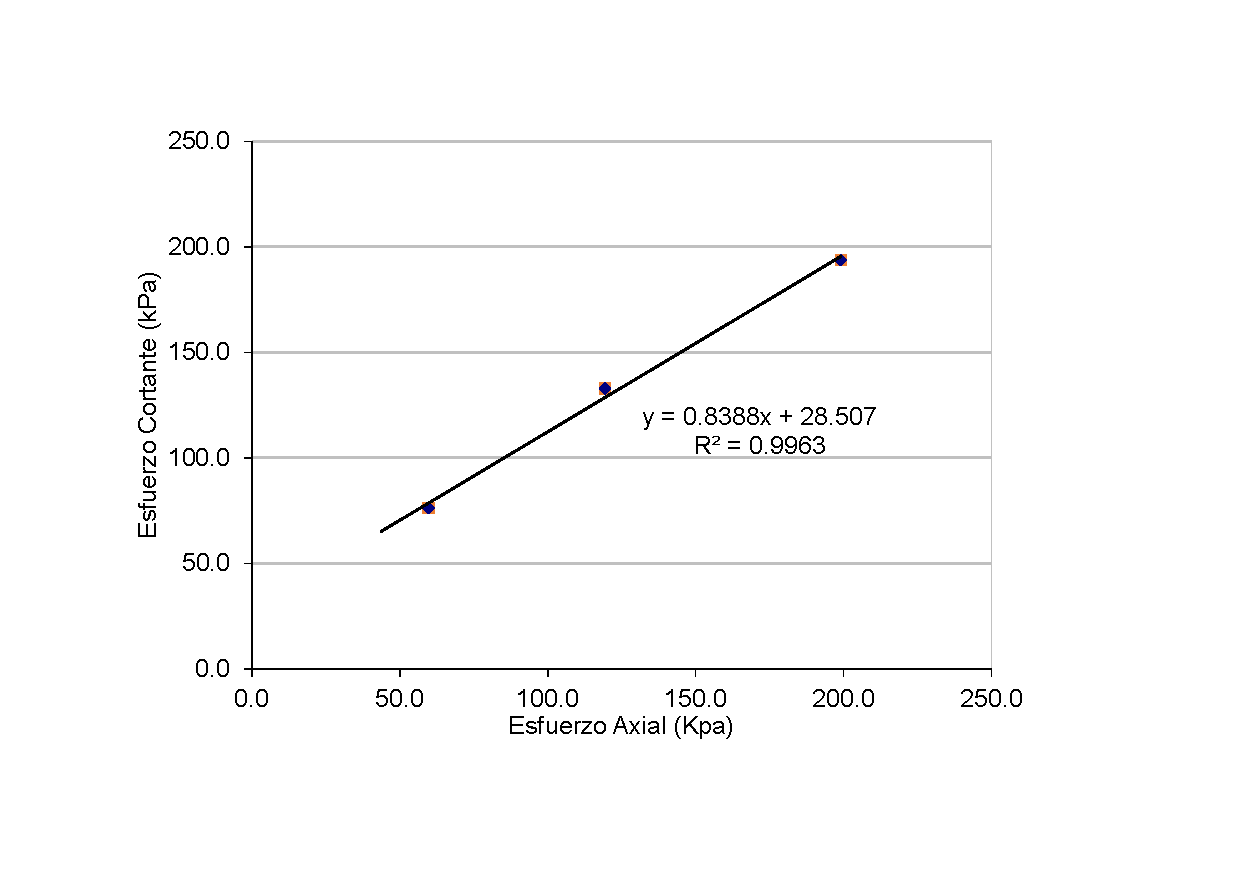
\includegraphics[trim={0 1.5cm 0 1.5cm},clip,scale=0.8]{img/line.pdf}
\caption{Estimaci\'on de par\'ametros de resistencia al corte basados en los datos de las muestras analizadas en la estaci\'on 1.}
\label{fig:line}
\end{figure}

\begin{table}[H]
\centering
\caption{Resultado de esfuerzo cortante para cada etapa de carga (Esfuerzo Axial) obtenida para las 3 muestras recolectadas en la estaci\'on 1.}
\begin{tabular}{|lc|cc}
\hline
\multicolumn{1}{|l|}{Muestra}                                                               & 1                       & \multicolumn{1}{c|}{2}     & \multicolumn{1}{c|}{3}     \\ \hline
\multicolumn{1}{|l|}{\begin{tabular}[c]{@{}l@{}}Esfuerzo Cortante\\   $\left( kPa \right) $\end{tabular}} & 76.2                    & \multicolumn{1}{c|}{132.8} & \multicolumn{1}{c|}{194}   \\ \hline
\multicolumn{1}{|l|}{Esfuerzo Axial $\left( kPa \right) $}                                                & 59.7                    & \multicolumn{1}{c|}{119.4} & \multicolumn{1}{c|}{199.1} \\ \hline
Angulo de Fricci\'on $  $                                                                      & \multicolumn{1}{l|}{40} & \multicolumn{1}{l}{}       & \multicolumn{1}{l}{}       \\ \cline{1-2}
Cohesi\'on $\left( kPa \right) $                                                                            & \multicolumn{1}{l|}{29} & \multicolumn{1}{l}{}       & \multicolumn{1}{l}{}       \\ \cline{1-2}
\end{tabular}
\label{table:line}
\end{table}

\begin{figure}[H]
\centering
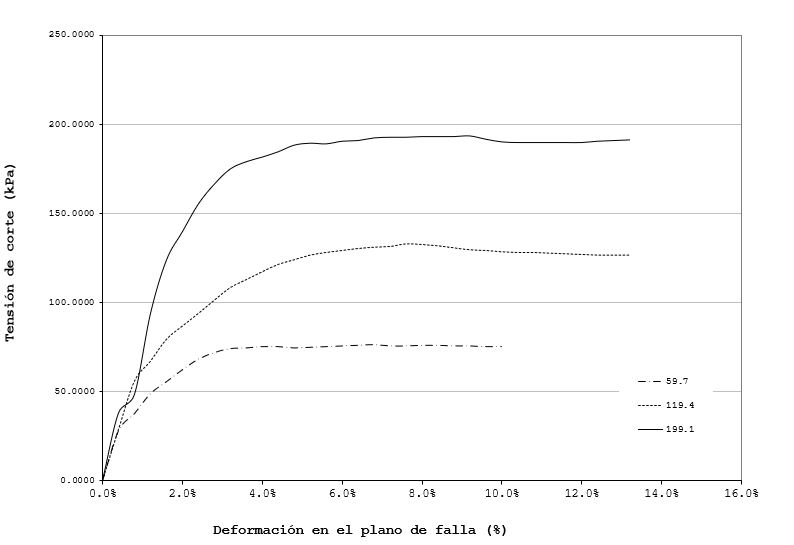
\includegraphics[scale=1]{img/diagramatd.JPG}
\caption{Diagrama tensi\'on deformaci\'on para las muestras de la estaci\'on 1. Se puede observar como se presenta un comportamiento pl\'astico al haber alcanzado un dial de deformaci\'on que se encuentra entre un   10\% y un 14\% del di\'ametro de la muestra.}
\label{fig:toma-bloque}
\end{figure}


\paragraph{Estaci\'on 2.}
Las muestras de los tuvos PCV recolectadas en la estaci\'on 2 recibieron la misma preparacion realizada sobre las muestras de la estaci\'on 1. Sin embargo al momento de realizar el ensayo de corte directo, se produjo una deformaci\'on inusual en este ensayo, provocando que un lado de la muestra cediera y se comprimiera m\'as que otro. Dicha deformaci\'on ocurr\'ia a lo largo de la ejecuci\'on del ensayo produciendo una deformaci\'on vertical progresiva a medida que se presentaba la deformaci\'on lateral producida por el esfuerzo cortante, invalidando los datos obtenidos. El procedimiento se reviso meticulosamente con ayuda del personal de laboratorio, obteniendo el mismo resultado en repetidas ocaciones. Motivo por el cual no fue posible obtener una envolvente para las muestras pertenecientes a dicha estaci\'on.

\begin{figure}[H]
\centering
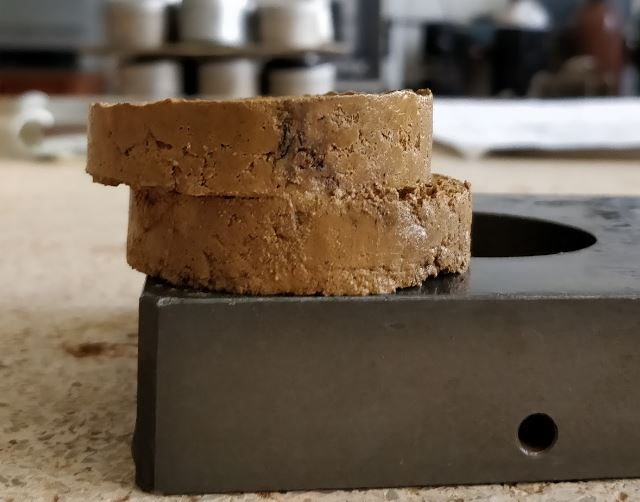
\includegraphics[scale=1]{img/est2.jpg}
\caption{Muestra recolectada de la estaci\'on 2 posterior al ensayo de corte directo. N\'otese la deformaci\'on anormal en la parte izquierda del fragmento superior de la muestra, el cual presenta un grado de compresi\'on mayor a su lado opuesto.}
\label{fig:toma-bloque}
\end{figure}


\paragraph{Scoops3D.}
Tomando los resultados de laboratorio expuestos anteriormente se procedi\'o a ingresar los valores correspondientes al \'angulo de fricci\'on, cohesi\'on y gravedad espec\'ifica en Scoops3D. Se mantuvo la configuraci\'on de caja de b\'usqueda descrita en la figura \ref{fig:test}.

\begin{figure}[H]
\centering
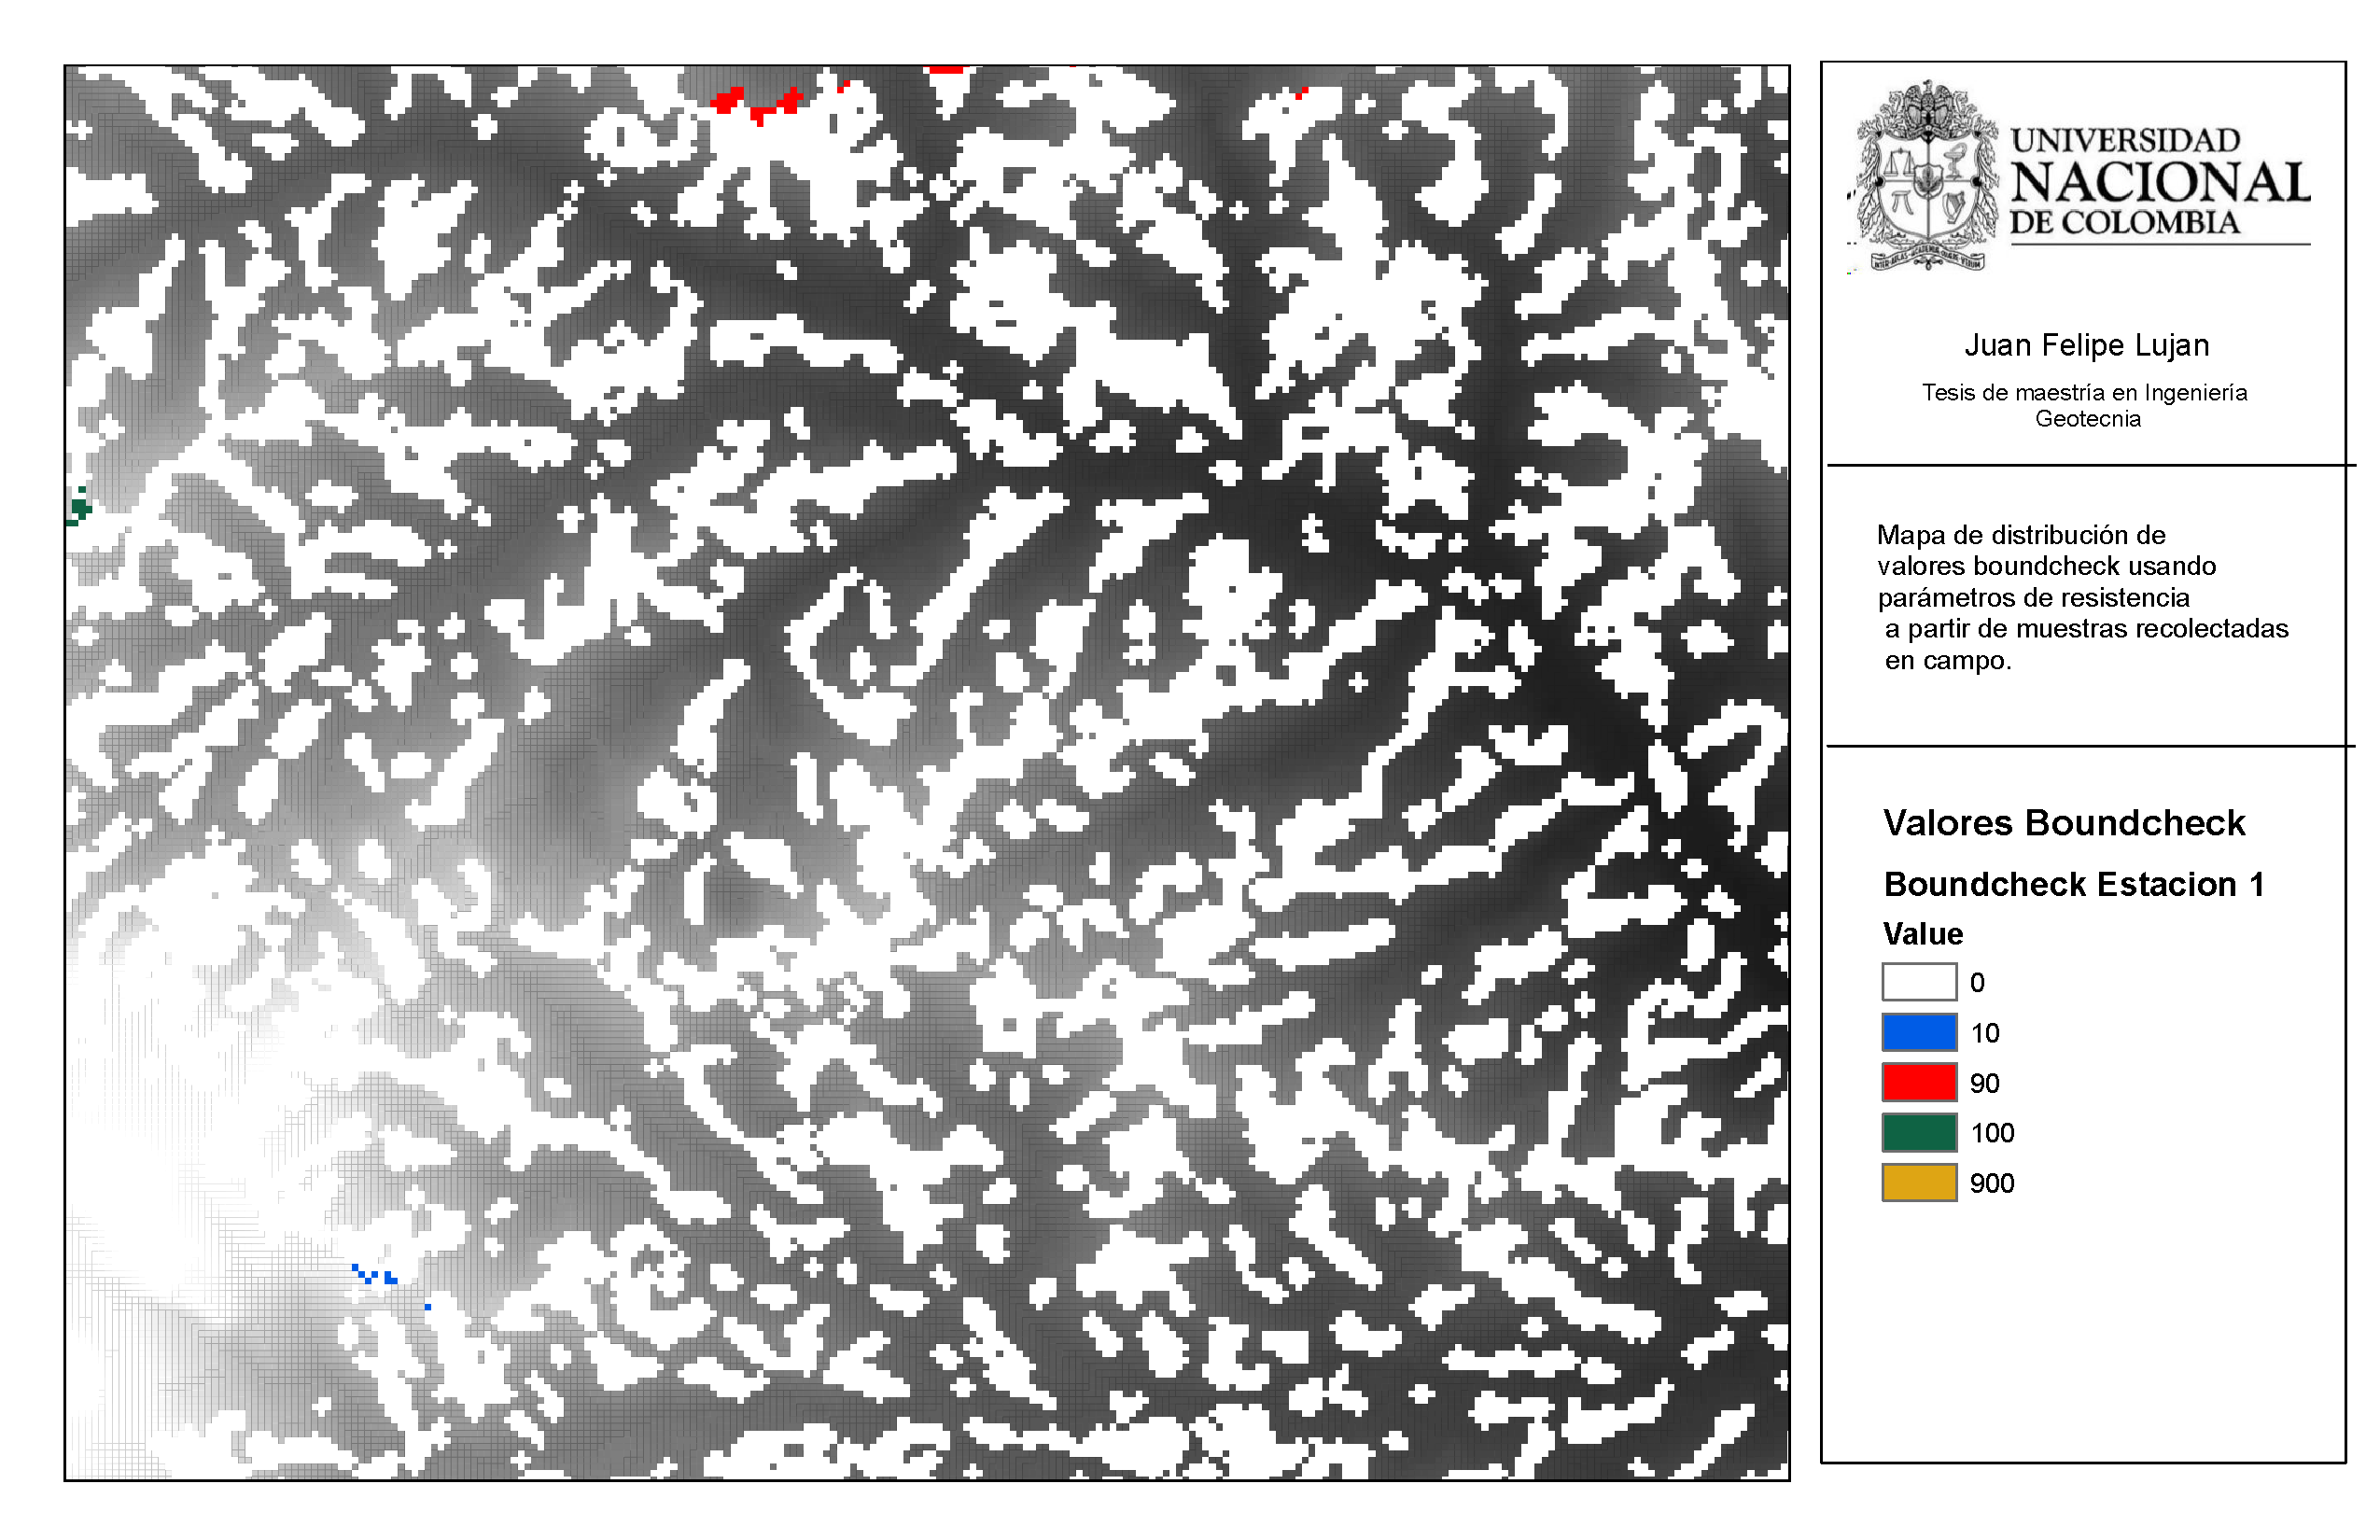
\includegraphics[scale=0.3]{img/boundcheckCampo.pdf}
\caption{Control de calidad a la corrida de Scoops3D con datos de campo por media del an\'alisis del archivo de salida Boundcheck. Fuente: Elaboraci\'on propia.}
\label{fig:dem usado}
\end{figure}

Se puede apreciar en el archivo de salida \textsf{boundcheck} que la caja de b\'usqueda propuesta en las pruebas preliminares es aplicable los datos obtenidos de las muestras recolectadas en campo. Dicho comportamento era esperado debido a la abundancia de pendientes pronunciadas en esta zona del municipio de Ciudad Bolivar.

Los p\'ixeles marcados con color azul en el sector suroccidental de la zona de trabajo indican que la extension de la caja de b\'usqueda hacia el extremo sur fue una limitante para aplicar el m\'etodo bishop (centro de la superficie de falla por fuera de la caja de b\'usqueda, en direccion sur) lo mismo ocurre con los pixeles marcados de color rojo hacia el extremo norte de la zona de trabajo (centro de la superficie de falla por fuera de la caja de b\'usqueda, en direccion norte)

Sin embargo, dado que la cuenta de p\'ixeles donde se presenta dicho comportamiento es de 89 sobre un total de 28057, se puede decir que la caja de b\'usqueda usada es aplicable en un 99.996\% a la zona de trabajo.
Para aumentar la cobertura ser\'ia necesario realizar pruebas en equipos de computo con mayores capacidades de computo a las descritas en el cap\'itulo 5.


\begin{figure}[H]
\centering
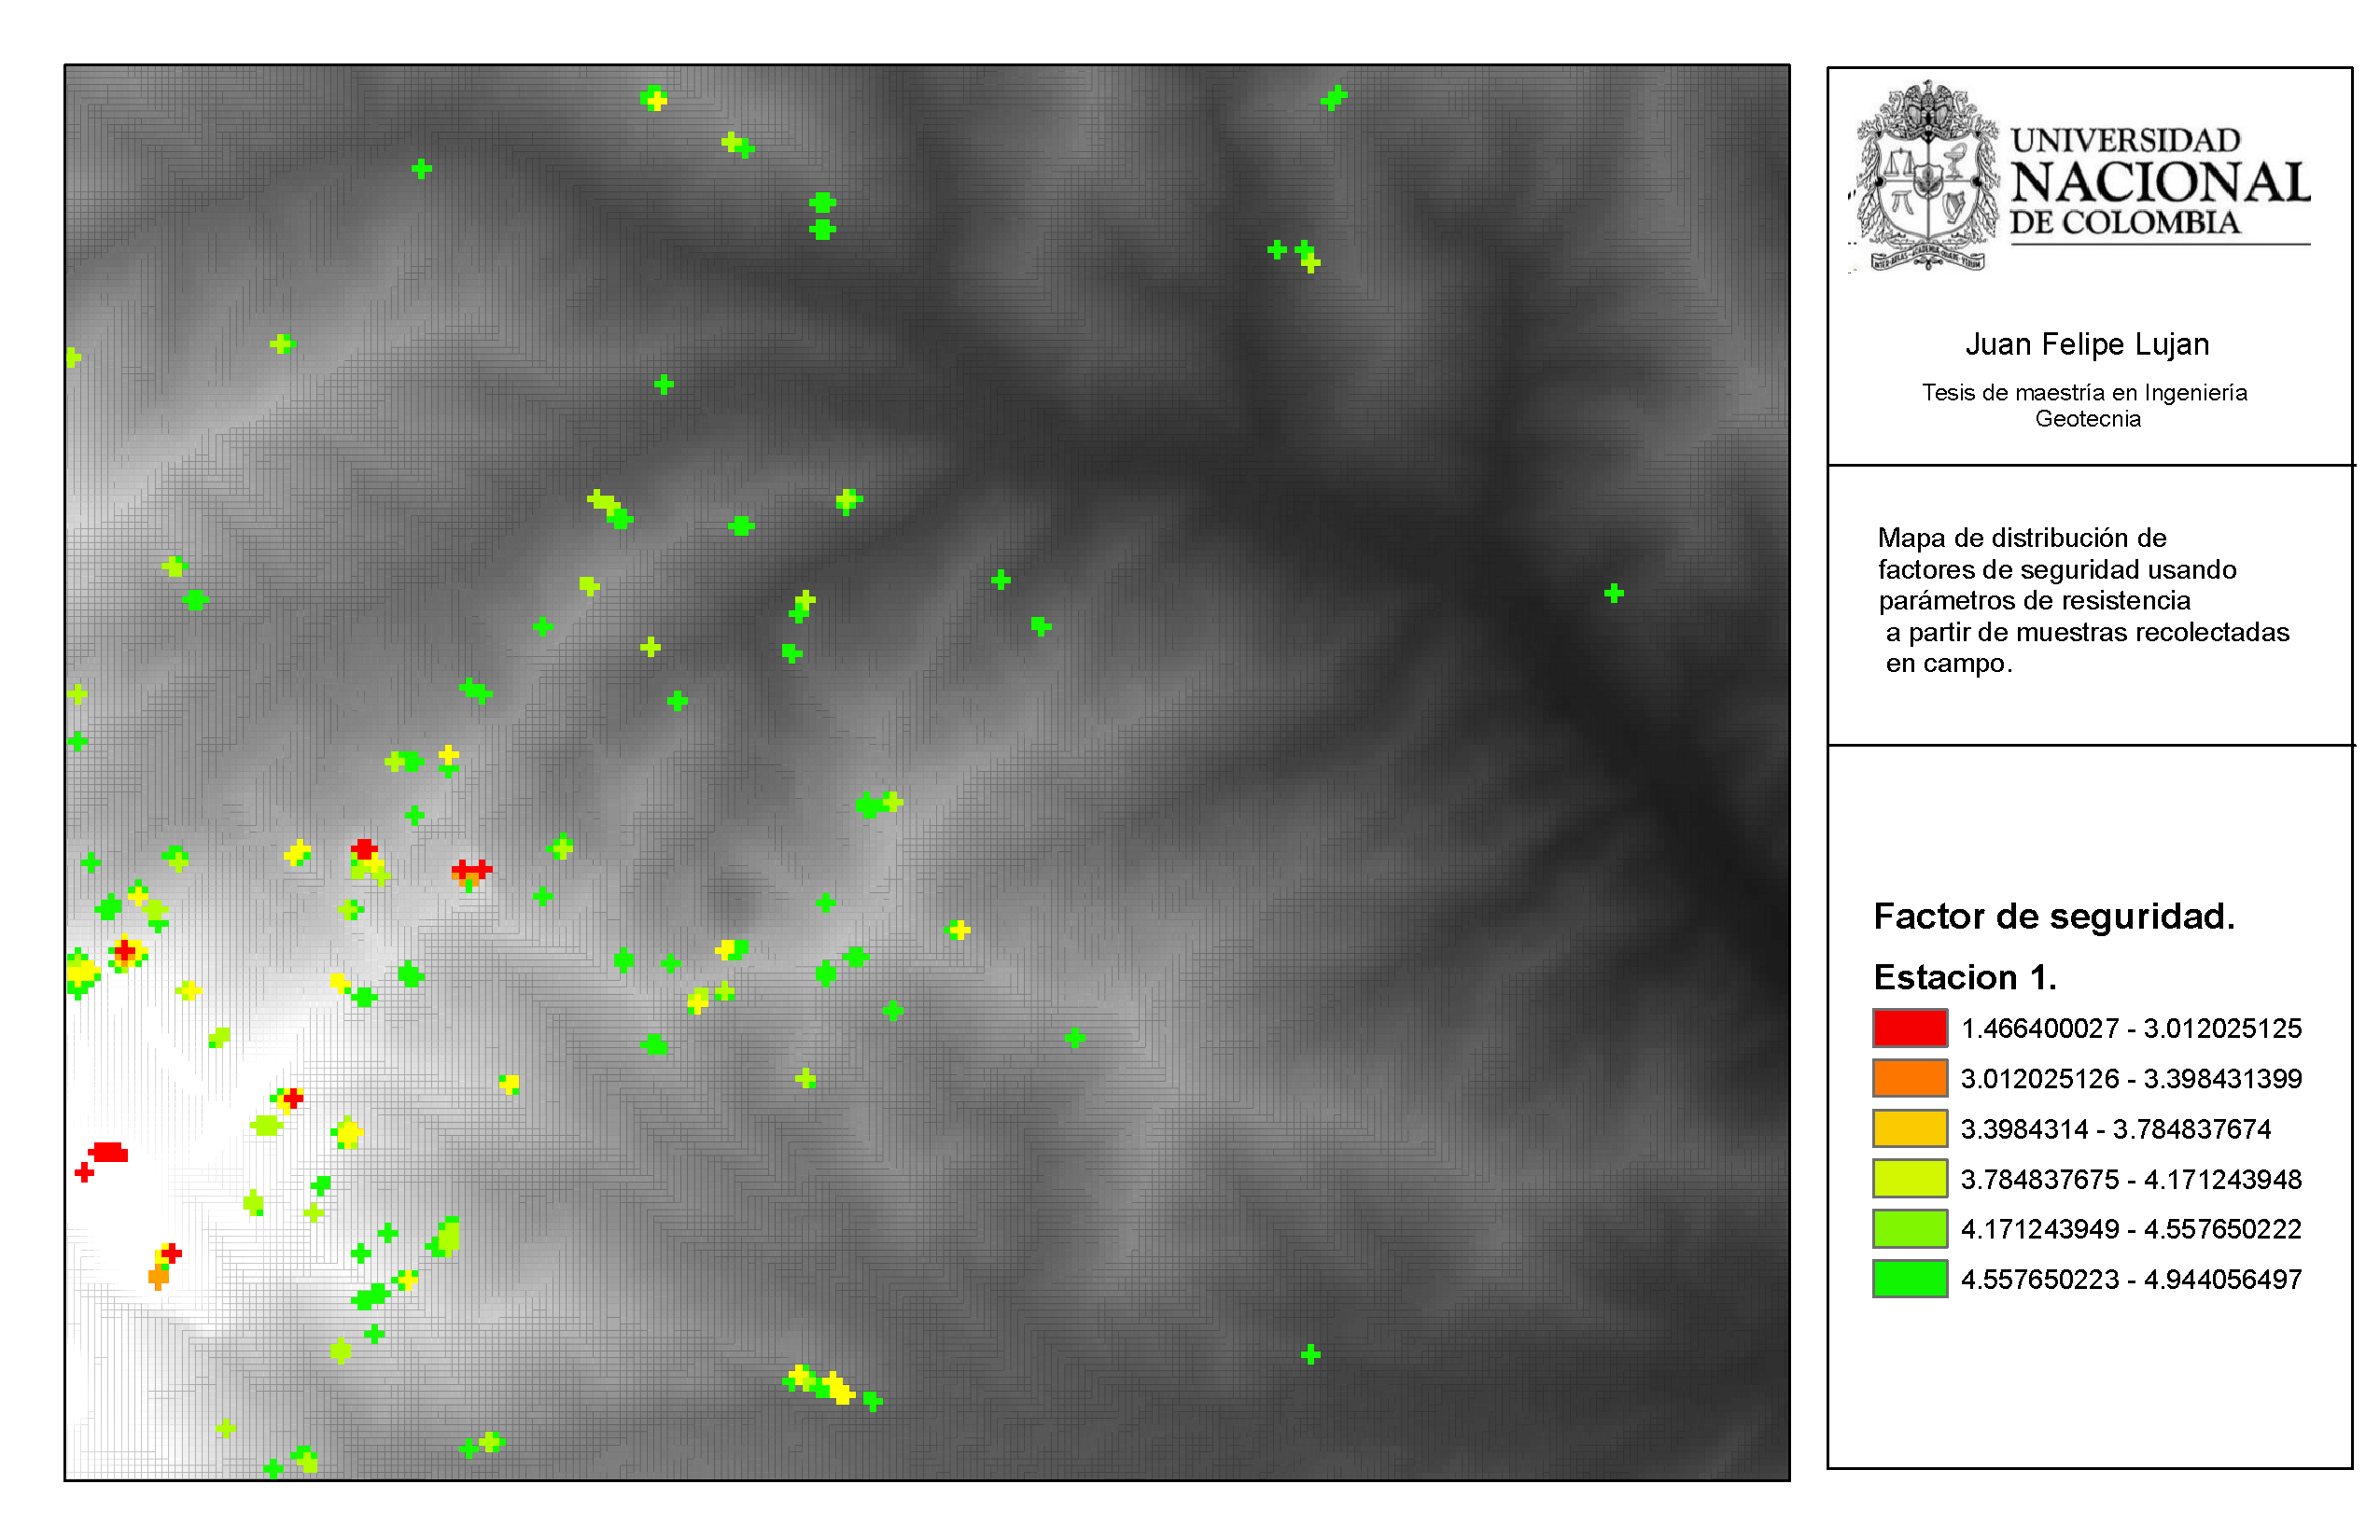
\includegraphics[scale=0.3]{img/fos3DCampo_coarse.pdf}
\caption{Resultado  de la ejecuci\'on de Scoops 3D usando la configuraci\'on usada en las pruebas preliminares (caja de b\'usqueda).}
\label{fig:fos3dout_coarse}
\end{figure}


Como resultado del an\'alisis probabil\'istico por medio del m\'etodo Bishop utilizando las valores de resistencia obtenidos en los an\'alisis de laboratorio realizadas a las muestras recolectadas del \'area de trabajo se obtiene el mapa de \emph{distribuciones de factores de seguridad} presentado en la figura \ref{fig:fos3dout_coarse}.
Donde se analizaron un total de \(1\,665\,954\) superficies de falla.

Se puede apreciar que, en los extremos sur occidental (a lo largo de las laderas que componen la cuenca de la quebrada La Linda) y norte de la zona de trabajo se presentan acumulaciones de lugares con disminucion de factores de seguridad los cuales var\'ian frecuentemente entre 3 y 5. Se expluye del an\'alisis la zona donde se localiza la formaci\'on Barroso.

El sector con menor valor de F se encuentra ligeramente al norte de la Formaci\'on Barroso(Kvb) donde los suelos de la Formaci\'on Penderisco alcanzan F de 1.91.  Mediante las m\'etricas de Scoops3D entregadas por Scoops3D se puede determinar que dicha zona est\'a compuesta por  $534.24\,\text{kg}$ de material y su v\'olumen es de $211.180\text{m}^{3}$


A\'un considerando un valor de F mayor a 3.0 , en la zona de trabajo se encontraron un total de 1280 p\'ixeles con \textit{F} inferior a este valor. Teniendo en cuenta que el \'area de cada p\'ixel es de  $1460.65\,\text{m}^{2}$ el \'area  equivalente bajo tal \textit{cutoff} es de $1'869,636 \text{m}^{2}$



\input{kap7/kap7}



\addcontentsline{toc}{chapter}{\numberline{}Bibliograf\'ia}
\bibliographystyle{plaindin_esp}
\bibliography{BibliMSc}
\end{document}